%%%%%%%%%%%%%%%%%%%%%%%%%%%%%%%%%%%%%%%%%%%%%%%%%%%%%%%%%%%%%%%%%%%%%%%%%%%%%%
% This is just an example/guide for you to refer to when submitting
% manuscripts to Frontiers, it is not mandatory to use Frontiers .cls files
% nor frontiers.tex  %
% This will only generate the Manuscript, the final article will be typeset by
% Frontiers after acceptance.
%
% When submitting your files, remember to upload this *tex file, the pdf
% generated with it, the *bib file (if bibliography is not within the *tex)
% and all the figures.
%%%%%%%%%%%%%%%%%%%%%%%%%%%%%%%%%%%%%%%%%%%%%%%%%%%%%%%%%%%%%%%%%%%%%%%%%%%%%%

%%% Version 3.4 Generated 2022/06/14 %%%
%%% You will need to have the following packages installed: datetime,
%%% fmtcount, etoolbox, fcprefix, which are normally inlcuded in WinEdt.
%%% In http://www.ctan.org/ you can find the packages and how to install them,
%%% if necessary.
%%% NB logo1.jpg is required in the path in order to correctly compile front
%%% page header

% for articles in journals using the Harvard Referencing Style (Author-Date),
% for Frontiers Reference Styles by Journal: https://zendesk.frontiersin.org/hc/en-us/articles/360017860337-Frontiers-Reference-Styles-by-Journal
\documentclass[utf8]{FrontiersinHarvard}
% for articles in journals using the Vancouver Reference Style (Numbered), for
% Frontiers Reference Styles by Journal: https://zendesk.frontiersin.org/hc/en-us/articles/360017860337-Frontiers-Reference-Styles-by-Journal
%\documentclass[utf8]{FrontiersinVancouver}
% Vancouver Reference Style (Numbered) for articles in the journals "Frontiers
% in Physics" and "Frontiers in Applied Mathematics and Statistics"
%\documentclass[utf8]{frontiersinFPHY_FAMS}

\usepackage{
    url,
    hyperref,
    lineno,
    microtype,
    subcaption,
    booktabs,
    paralist,
    tablefootnote,
    natbib
}

\usepackage[onehalfspacing]{setspace}

%%%%%%%%%%%%%%%%%%%%%%%%%%%%%%%%%%%%%%%%%%%%%%%
% Code listings
%%%%%%%%%%%%%%%%%%%%%%%%%%%%%%%%%%%%%%%%%%%%%%%
\usepackage{inconsolata}

% Code listings with package minted. Requires python
%   pyenv virtualenv 3.x.x myenv
%   pyenv activate myenv
%   pip install pygments
% Then add compilation flag -shell-escape
\usepackage[outputdir=out,newfloat]{minted}
%\usepackage[outputdir=out]{minted}

\usepackage[skins, breakable]{tcolorbox}
\tcbuselibrary{minted}

% Code listing, e.g.
%
%     \begin{codelisting}{
%         \texttt{update} method of the networked audio client implementation,
%         minted style=xcode,
%         minted language=cpp,
%         label=ls:njc-update,
%         float=h!
%     }
%         void NetJUCEClient::update(void) {
%             doAudioOutput();
%
%             handleAudioInput();
%         }
%     \end{codelisting}
\newtcblisting[auto counter]{codelisting}[1]{%
    enhanced,
%    breakable,
%    colback=backcolour,
%    colframe=captioncolor,
    fonttitle=\bfseries\normalsize,
    listing only,
    sharp corners,
    bottomrule=1pt,
    toprule=2pt,
    leftrule=0pt,
    rightrule=0pt,
    title=Listing \thetcbcounter: #1,
    minted style=xcode,
    minted options={
        fontsize=\scriptsize,
        autogobble
    }
}

% Input code from file, e.g.
%
%       \codeinputlisting[float=h]
%          {text}
%          {listings/udp-packet.txt}
%          {Network capture: ethernet frame containing a UDP packet}
%          {packet-hello-world}
\newtcbinputlisting[use counter from=codelisting]{\codeinputlisting}[5][]{
    minted language=#2,
    listing file={#3},
    title=Listing \thetcbcounter: #4,
    label=listing:#5,
    enhanced,
%    breakable,
%    colback=backcolour,
%    colframe=captioncolor,
    fonttitle=\bfseries\normalsize,
    listing only,
    sharp corners,
    bottomrule=1pt,
    toprule=2pt,
    leftrule=0pt,
    rightrule=0pt,
    minted style=xcode,
    minted options={
        fontsize=\scriptsize,
        autogobble
    },#1
}

%%%%%%%%%%%%%%%%%%%%%%%%%%%%%%%%%%%%%%%%%%%%%%%%
% SI Units
%%%%%%%%%%%%%%%%%%%%%%%%%%%%%%%%%%%%%%%%%%%%%%%%
\usepackage{siunitx}
\sisetup{detect-all}

%%%%%%%%%%%%%%%%%%%%%%%%%%%%%%%%%%%%%%%%%%%%%%%%
% TODOS
%%%%%%%%%%%%%%%%%%%%%%%%%%%%%%%%%%%%%%%%%%%%%%%%
\usepackage[
    disable, %turn off todonotes
    colorinlistoftodos, %enable a coloured square in the list of todos
    textwidth=\marginparwidth, %set the width of the todonotes
    textsize=scriptsize, %size of the text in the todonotes
]{todonotes}


\def\keyFont{\fontsize{8}{11}\helveticabold }

% Internal refs
\newcommand{\figref}[1]{Figure~\ref{#1}}
\newcommand{\figsref}[2]{Figures~\ref{#1} and~\ref{#2}}
\newcommand{\tabref}[1]{Table~\ref{#1}}
\newcommand{\secref}[1]{section~\ref{#1}}
\newcommand{\Secref}[1]{Section~\ref{#1}}
\newcommand{\lstref}[1]{Listing~\ref{#1}}

% Number with base 10 postfix subscript
\newcommand{\numDec}[1]{\num{#1}\textsubscript{10}}

%%%%%%%%%%%%%%%%%%%%%%%%%%%%%%%%%%%%%%%%%%%%%%%%
% Math definitions
%%%%%%%%%%%%%%%%%%%%%%%%%%%%%%%%%%%%%%%%%%%%%%%%
\newcommand{\bfx}{\mathbf{x}}
\newcommand{\Sigin}{\hat{S}_{\text{in}}}
\newcommand{\sigin}{\hat{s}_{\text{in}}}
\newcommand{\sigink}{\hat{s}_{\text{in},k}}

% use et al only if is more than 1 author
\def\firstAuthorLast{Rushton {et~al.}}
\def\Authors{Thomas Albert Rushton\,$^{1,*}$, Romain Michon\,$^{1}$, Stefania
Serafin\,$^{2}$ Tanguy Risset\,$^{1}$ and Stéphane Letz\,$^{3}$}
% Affiliations should be keyed to the author's name with superscript numbers
% and be listed as follows: Laboratory, Institute, Department, Organization,
% City, State abbreviation (USA, Canada, Australia), and Country (without
% detailed address information such as city zip codes or street names).
% If one of the authors has a change of address, list the new address below
% the correspondence details using a superscript symbol and use the same
% symbol to indicate the author in the author list.
\def\Address{
    $^{1}$Inria, INSA Lyon, CITI, EA3720, 69621 Villeurbanne, France \\
    $^{2}$Aalborg University, A. C. Meyers Vænge 15, 2450 Copenhagen, Denmark \\
    $^{3}$GRAME-CNCM, INSA Lyon, Inria, CITI, EA3720, 69621 Villeurbanne, France
}
% The Corresponding Author should be marked with an asterisk
% Provide the exact contact address (this time including street name and city
% zip code) and email of the corresponding author
\def\corrAuthor{Corresponding Author}

\def\corrEmail{thomas.rushton@inria.fr}


% Show line numbers
\linenumbers

\begin{document}
    \onecolumn
    \firstpage{1}

    \title[Networked Microcontrollers for Accessible, Distributed Spatial Audio]
    {Networked Microcontrollers for Accessible, Distributed Spatial Audio}

    \author[\firstAuthorLast ]{\Authors}
    \address{}
    \correspondance{}

    % If there is more than 1 corresponding author, comment this line and
    % uncomment the following one.
    \extraAuth{}
%\extraAuth{corresponding Author2 \\ Laboratory X2, Institute X2, Department X2, Organization X2, Street X2, City X2 , State XX2 (only USA, Canada and Australia), Zip Code2, X2 Country X2, email2@uni2.edu}

    \maketitle

    \begin{abstract}

%%% Leave the Abstract empty if your article does not require one, please see
%%% the Summary Table for full details.
        \section{}

%    For full guidelines regarding your manuscript please refer to
%    \href{http://www.frontiersin.org/about/AuthorGuidelines}{Author Guidelines}.
%
%    As a primary goal, the abstract should render the general significance and
%    conceptual advance of the work clearly accessible to a broad readership.
%    References should not be cited in the abstract.
%    Leave the Abstract empty if your article does not require one, please see
%    \href{http://www.frontiersin.org/about/AuthorGuidelines#SummaryTable}{Summary Table}
%    for details according to article type.

        State-of-the-art systems for spatial and immersive audio are typically very
        costly, being reliant on specialist audio hardware capable of performing
        computationally intensive signal processing and delivering output to many
        tens, if not hundreds, of loudspeakers.
        Centralised systems of this sort suffer from limited accessibility due to
        their inflexibility and expense.
        Building on the research of the past few decades in the transmission of
        audio data over computer networks, and the emergence in recent years of
        increasingly capable, low-cost microcontroller-based development platforms
        with support for both networking and audio functionality, we present a
        prototype decentralised, modular alternative.
        Having previously explored the feasibility of running a microcontroller
        device as a networked audio client, here we describe the development of a
        client-server system with improved scalability via multicast data
        transmission.
        The system operates on ubiquitous, commonplace computing and networking
        equipment, with a view to it being a simple, versatile, and
        highly-accessible platform, capable of granting users the freedom to explore
        audio spatialisation approaches at vastly reduced expense.
        Though faced by significant technical challenges, particularly with regard
        to maintaining synchronicity between distributed audio processors,
        the system produces perceptually plausible results.
        Findings are commensurate with a capability, with further development
        and research, to disrupt and democratise the fields of spatial and immersive
        audio.

        \tiny
        \keyFont{ \section{Keywords:}\label{sec:keywords}
        Spatial audio,
            Networked audio,
            Distributed systems,
            Wave Field Synthesis,
            Microcontroller,
            Accessibility
%        keyword,
%        keyword,
%        keyword
        } %All article types: you may provide up to 8 keywords; at least 5 are mandatory.
    \end{abstract}

    Word-count: 11868; tables: 1; figures: 13.

    \section{Introduction}\label{sec:introduction}

    Recent developments in virtual and augmented reality technologies and
    object-based audio~\citep{geier_object-based_2010} have led to an
    acceleration in interest in the synthesis of virtual sound fields via
    approaches such as Wave Field Synthesis (WFS) and Higher Order Ambisonics
    (HOA)~\citep{berkhout_acoustic_1993,ahrens_theory_2008,daniel_further_2003,
        frank_producing_2015}.
    These techniques call for the deployment of large numbers of loudspeakers,
    and \textit{in situ} installations of dedicated hardware and software.
    The costs associated with such installations have seen them largely
    restricted to the preserve of concert venues, cinemas, and institutions with
    the means to purchase and operate large-scale systems of this sort.

    Advancements in embedded computing mean that there now exist an assortment
    of small, low-cost devices with support for audio Digital Signal Processing
    (DSP).
    These devices are relatively easy to program with open-source APIs and
    libraries, and may provide support for communication over ubiquitous
    computer networking equipment and protocols, an important capability in
    light of the rise of high-speed ethernet as a standard for multichannel
    audio transmission~\citep{bakker_introduction_2014}.
    A network of such devices could be used to \textit{distribute} the problem
    of audio spatialisation, permitting a modular, scalable approach that could
    lower the barrier to entry to what is otherwise a comparatively exclusive
    branch of audio research.
    Potential applications of such a system... auralisation, virtual
    acoustics... a distributed system could afford an overall increase in
    available computing power to support auralisation algorithms that require
    the computation of expensive convolutions~\citep{}.

    \begin{figure}[ht]
        \centering
        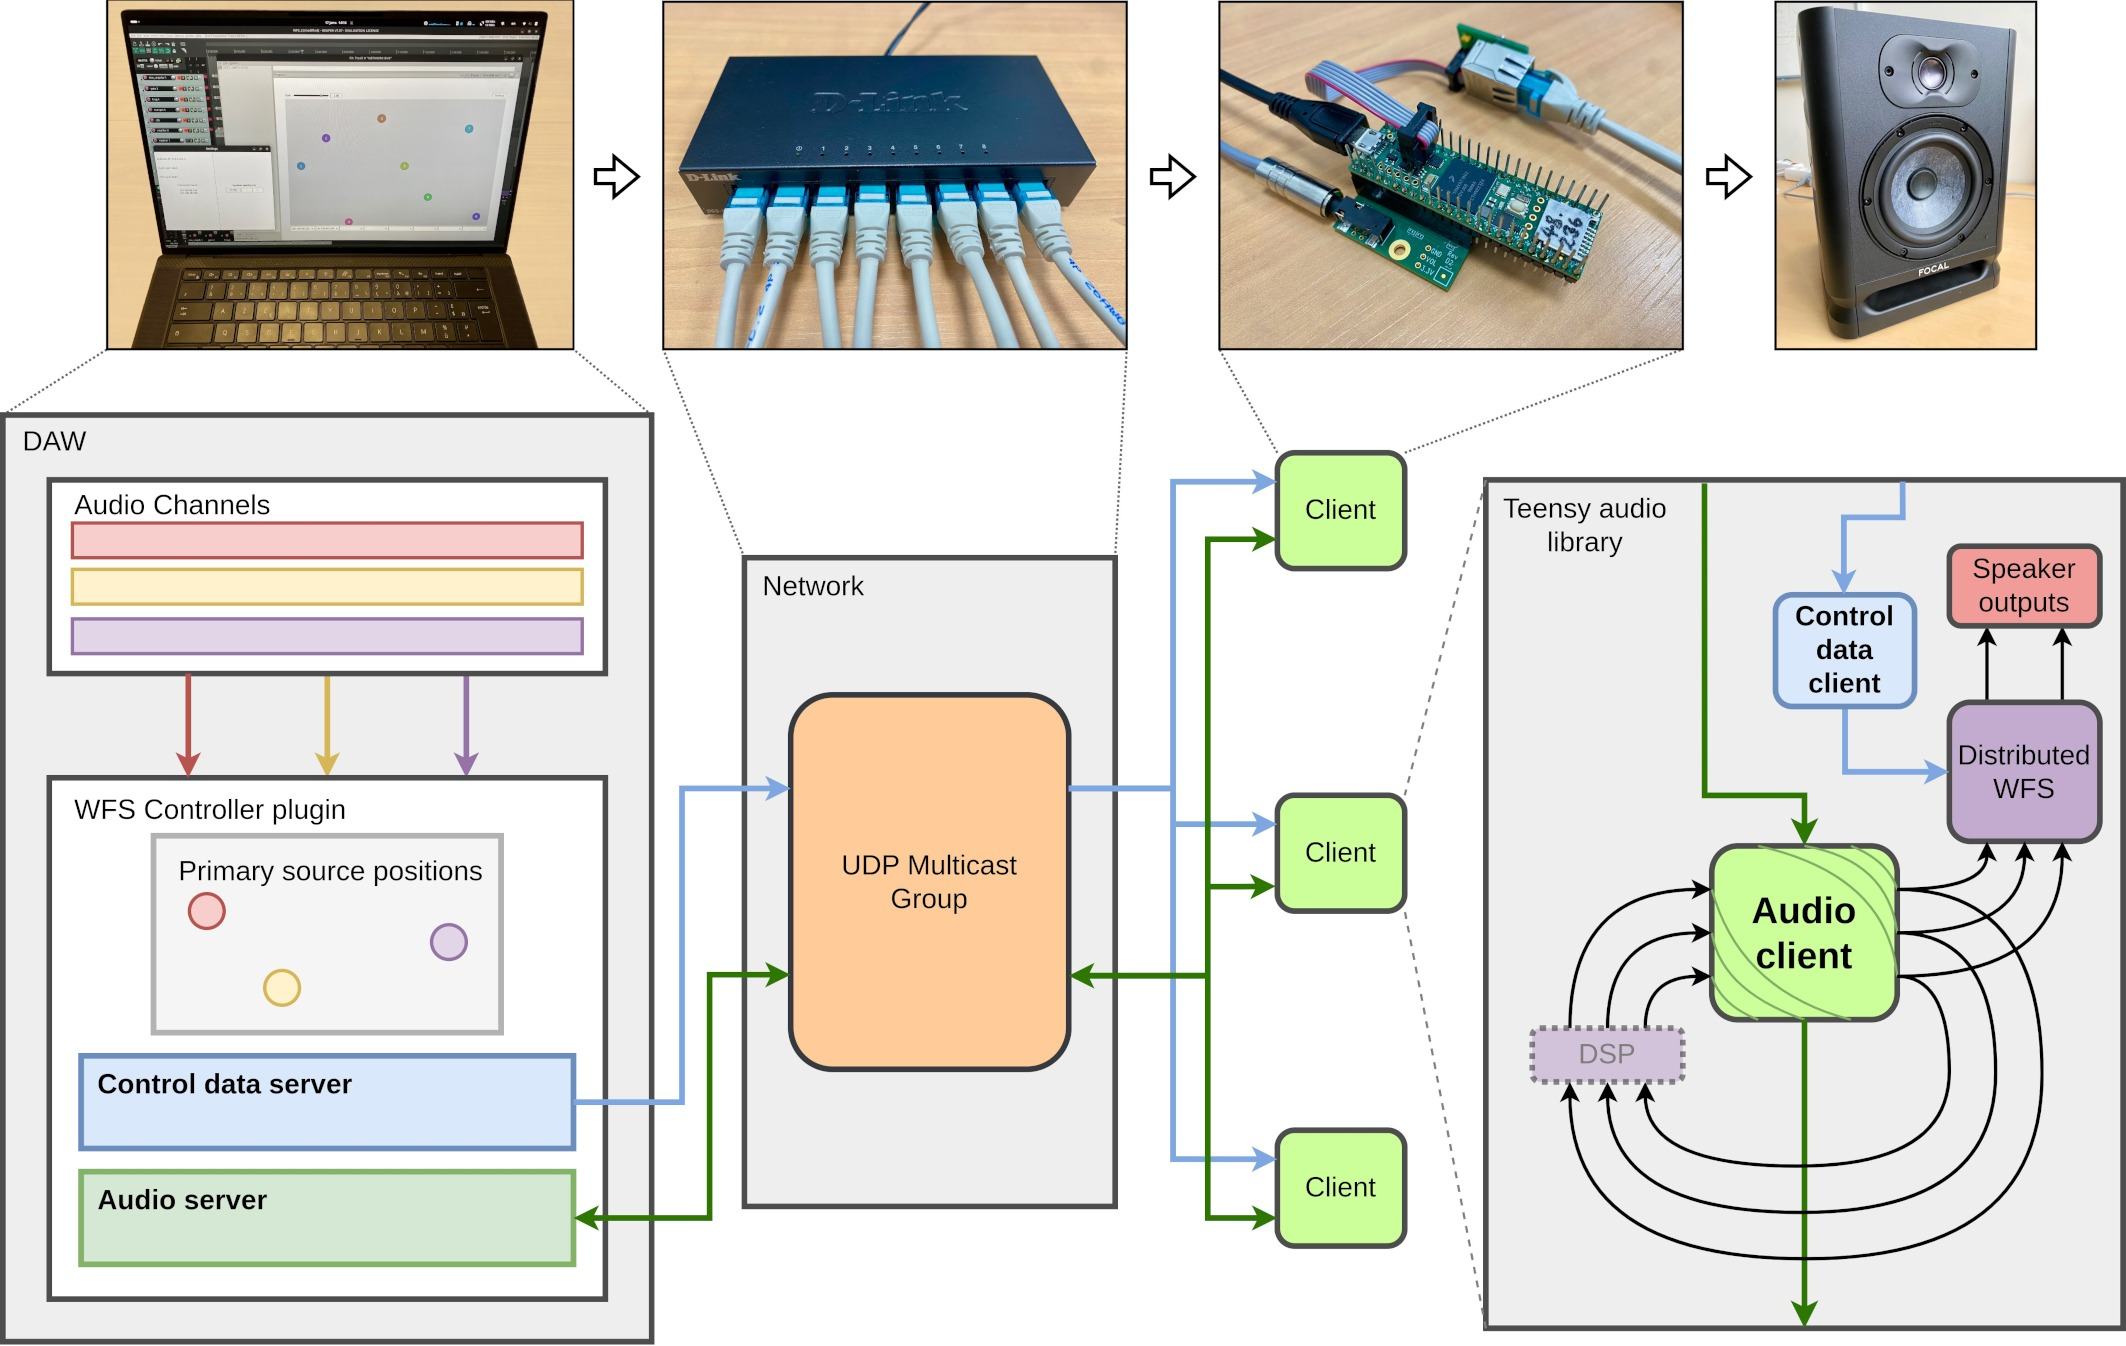
\includegraphics[width=\textwidth]{figures/system_overview}
        \caption{
            Overview of the proposed distributed, networked audio system.
            A general purpose computer runs DAW software, which in turn runs an
            instance of an audio plugin that encapsulates servers for audio and
            control data.
            The computer is physically connected, via a network switch, to
            microcontroller-based clients.
            The clients receive the audio and control data, which are delivered
            to a distributed audio spatialisation algorithm, and return an audio
            stream to the server (perhaps via some manner of signal processor).
            Clients deliver the output signals produced by their instance of the
            distributed algorithm to loudspeakers.
        }
        \label{fig:system-overview}
    \end{figure}

    In this article we describe the development of a distributed system for
    spatial and immersive audio.
    In \secref{sec:background} we discuss the technological and scholarly
    background to this project, including developments in networked audio and
    embedded hardware platforms, spatial audio techniques, and distributed audio
    systems.
    Building upon this background, and prior work on a microcontroller-based
    networked audio client~\citep{rushton_microcontroller-based_2023},
    \secref{sec:method} details the development of the proposed system, an
    overview of which is depicted in \figref{fig:system-overview}.
    With a view to optimising accessibility and interoperability with existing
    audio tools, the system's server component is encapsulated in an audio
    plugin suitable for use in a Digital Audio Workstation (DAW)\@.
    The server delivers audio and control data to a network of
    microcontroller-based clients via a local area network, and clients,
    programmed with a parallelised spatial audio algorithm, use the audio and
    control data to perform their part of the distributed signal process.
    Minimising inter-client asynchronicity in a distributed audio context is the
    most significant technical problem, and the network client implementation
    incorporates strategies for addressing this challenge.

    The previous system was not formally evaluated, but, anecdotally, provided
    support for the \textit{holophonic} effect of wave field synthesis.\
    A perceptual evaluation of the new system was conducted, and this is
    described, along with a technical evaluation, in \secref{sec:results}.
    Finally, in \secref{sec:conclusion}, we give an overview of our findings to
    date and describe our ambitions for future work.

    \section{Background}\label{sec:background}

    \dots

    \subsection{Networked Audio}\label{subsec:networked-audio}

    The transmission of audio data has been a topic of research interest since the
    earliest days of computer networking as it is recognised today, i.e.\ over
    packet-switched networks, whereby data to be transmitted is grouped into
    packets \textemdash{} or ``datagrams'' \textemdash{} each consisting of a header
    and a payload.
    Voice transmission over ARPANET was being conducted as early as
    1974~\citep{schulzrinne_voice_1992} and the first standard for voice
    communication over packet-switched networks \textemdash{} the Network Voice
    Protocol (NVP) \textemdash{} was released in
    1977~\citep{cohen_specifications_1977}.

    The NVP standard, with control messages for `calling' and `ringing', was
    clearly intended for digital telephony, and communication was the primary
    focus of networked audio research well into the 1990s.
    Efforts on supporting real-time voice communication over wide area networks
    (WAN) centred on \textit{quality of service} (QoS), particularly with regard
    to the perennial issues of latency, packet loss, and network jitter
    \textemdash{} inconsistencies in the rate of packet
    transmission~\citep{hardman_reliable_1995,hardman_successful_1998}.
    Work at this time dealt with streams of compressed audio data, and speech
    coding algorithms to overcome the deleterious effects of dropped packets
    over unreliable network paths and low-bandwidth connections.

    Whereas the priority for digital telephony, and later voice over IP (VoIP)
    systems, is intelligibility, for musical purposes fidelity is of greater
    concern.
    The late 1990s, with the increasing availability of high-speed internet
    connections, saw the beginning of research into transmitting uncompressed audio
    data over the internet~\citep{chafe_simplified_2000,xu_real-time_2000}.
    Work of this sort was spearheaded by the \textit{SoundWIRE} project, developed
    by researchers at McGill University and Stanford University, and took the form
    of a wide variety of experiments with high quality audio over both WAN and local
    area networks (LAN).
    These experiments included LAN-based real-time musical
    performances~\citep{chafe_simplified_2000}, concert streaming over
    WAN~\citep{xu_real-time_2000,chafe_simplified_2000}, and sonification of QoS via
    a distributed digital waveguide dubbed the
    \textit{Network Harp}~\citep{chafe_simplified_2000,chafe_physical_2002}

    \subsubsection{Protocols and Systems}\label{subsubsec:protocols-systems}

    VoIP research in the 1990s focused on audio codecs and data
    compression~\citep{turletti_inria_1994,hardman_successful_1998}, seeking a
    compromise with the \textit{best-effort} nature of internet service.
    The SoundWIRE project, in search of high audio quality, turned its attention
    directly to the basic transport layer protocols of the Internet Protocol suite:
    Transmission Control Protocol (TCP) and User Datagram Protocol (UDP).
    Chafe et al.\ characterised their compression-free system as taking a
    ``simplified approach'' to networked audio~\citep{chafe_simplified_2000},
    emphasising the importance of delivering multichannel audio of at least CD
    quality (16-bit, \qty{44.1}{\kHz}) with as little latency as possible.

    SoundWIRE experiments included TCP-based concert streaming.
    TCP's \textit{connection-oriented}, one-to-one design enables packet flow
    control mechanisms that guarantee packet ordering and protect against
    against packet loss~\citep{schiavoni_alternatives_2013,
        al-dhief_performance_2018};
    at the expense of increased latency, these mechanisms safeguard quality of
    service, and thus audio fidelity; ideal for a remote concert scenario.
    UDP by comparison provides no such safeguards, but equally none of the
    associated computational or temporal overhead.
    Further, due to its \textit{connectionless} model, \textit{many-to-many}
    (multicast) and \textit{one-to-many} (broadcast) modes of transmission are
    possible via address spaces reserved as part of the internet protocol
    standard~\citep{meyer_iana_2010}.
    Via UDP, SoundWIRE was able to run as a distributed digital waveguide over a
    WAN spanning around \qty{4500}{\km}~\citep{chafe_simplified_2000}.

    From the SoundWIRE project emerged \textit{JackTrip}~\citep{
        caceres_jacktrip_2010,caceres_jacktripsoundwire_2010}, a hybrid system
    that couples a TCP handshake with audio transmission over UDP, thus
    sidestepping the overhead of TCP packet flow control.
    Rather than relying on TCP's built-in mechanisms for stream integrity,
    JackTrip supplements UDP with a number of optional buffering strategies that
    aim to optimise its operation in various network conditions.
    In this sense it is more flexible than TCP, but in effect JackTrip moulds
    UDP transmission into something akin to the connection-oriented model of
    TCP, and, in its `hub server' mode, into a kind of
    \textit{multiple one-to-one} design \textemdash{} multicast transmission is
    not possible.

    UDP has emerged as the protocol of choice for platforms enabling remote
    musical collaboration, serving as the basis for
    NetJACK~\citep{carot_netjack_2009}, part of the JACK Audio Connection Kit (a
    cross-platform audio host), the audiovisual performance streaming platform
    LOLA~\citep{drioli_networked_2013}, Jamulus~\citep{fischer_case_2015},
    Soundjack~\citep{renaud_networked_2007}, and other jamming-focused
    platforms, plus more recent entrants, the closed-source, but ultimately
    UDP-based Elk OS~\citep{turchet_elk_2021} for instance.
    UDP also plays a fundamental role in networked media streaming, being the
    typical transport-layer protocol behind the Real-time Transport Protocol
    (RTP), and it features in proprietary networked audio systems such as Dante
    (Digital Audio Network Through Ethernet)~\citep{dante_what_2022}.

    \subsubsection{AoE in the Audio Industry}

    In parallel with the work being carried out in academia on SoundWIRE, JackTrip
    and NetJACK, audio industry bodies \textemdash{} the IEEE (Institute of
    Electrical and Electronics Engineers) and AES (Audio Engineering Society)
    standards groups, and companies like Audinate, the creators of Dante
    \textemdash{} were taking an interest in networked audio.
    Traditional large-scale audio systems such as those used in broadcast, concert
    venues and recording studios rely on the installation of unwieldy combinations
    of analogue hardware and cabling, with many potential points of failure.
    Seeking literally to lighten the load posed by ``hundreds of
    kilograms''~\citep{bakker_introduction_2014} of cabling in analogue audio
    installations, in the 2000s audio companies were looking to high speed ethernet
    as a means to simplify the provision of high-quality, multichannel audio in
    industry settings.

    Key to these efforts was the release, in 2002, of the IEEE 1588 standard for
    the Precision Time Protocol (PTP), a means by which networked computer
    systems can achieve clock synchronicity~\citep{edison_ieee-1588_2002}.
    PTP (another protocol that typically uses UDP for transport) superseded the
    lower-resolution Network Time Protocol (NTP), and, under ideal conditions,
    can achieve synchronisation accuracy of sub-microsecond
    order~\citep{tongzhou_research_2022}.
    Synchronisation is achieved via the exchange of timestamped packets, coupled
    with precise estimates for send and receive times.
    Precision is best when timestamps can be calculated at the \textit{physical
    layer} \textemdash{} layer 1 of the Open Systems Interconnection (OSI)
    model, of which the aforementioned transport layer (layer 3) is a component
    \textemdash{} i.e.\ by dedicated timers at the level of the physical network
    interface.
    Legacy and low-cost networking equipment do not possess support for hardware
    timestamping, however~\citep{correll_design_2005}, and devices that do offer
    such support are markedly more expensive.\footnote{
        Consumer-grade, eight-port ethernet switches can cost as little as
        \texteuro{20};
        The cheapest equivalent devices with PTP support cost, at the time of
        writing, on the order of \texteuro{150-200}, e.g.\
        \url{https://www.fs.com/de-en/products/148180.html} \textemdash{} All
        URLs verified 12/01/2024.
    }
    PTP can be deployed as a software-only
    implementation~\citep{correll_design_2005}, albeit with impaired accuracy
    and a protracted clock-convergence period.

    Dante, with its promise of low-latency, highly-multichannel audio over wired
    LAN, and device synchronisation via hardware PTP, has become the de facto
    industry standard in networked audio~\citep{bakker_introduction_2014}.
    Bakker et al.\ refer to Dante as an ``open'' system, which is true, perhaps,
    in the sense that companies can incorporate the Dante system into their
    products under licence from Audinate;
    from the perspective of the academic community, however, Dante is very much
    a closed-source initiative and not a suitable platform for research.

    In 2011, IEEE released the Audio Video Bridging (AVB, IEEE 802.1)
    standard~\citep{ieee_ieee_2011}, and AES67 followed in
    2013~\citep{hildebrand_aes67-2013_2014}.
    These open technical standards describe \textit{suites} of protocols for
    tasks such as media transmission, device discovery and
    synchronisation, and interoperability with other systems.
    Both employ PTP for device synchronisation; AES67 uses RTP for media
    transmission, whereas AVB uses the data-link layer (layer 2) Audio Video
    Transport Protocol.
    Open implementations of AVB and AES67 exist, but, being complex standards
    featuring many components, such implementations may not be complete, support
    for embedded platforms is limited,\footnote{
        See, for example, \url{https://github.com/tschiemer/aes67} and
        \url{https://github.com/adiknoth/Open-AVB}.
    } and a reliance on
    PTP raises the barrier to entry.
    Ultimately, if an accessible solution is sought, attention must be turned
    back to the transport layer, and to UDP directly.

    \subsubsection{Challenges Posed by Networked Audio}\label{subsubsec:challenges}

    Time, especially when dealing with the fine margins posed by real-time audio
    processing, represents the principal source of difficulty in a networked
    audio setting.

    \textit{Jitter} refers to fluctuations in the rate of transmission or
    processing.
    In a networked audio setting, jitter gives rise to a situation whereby the
    arrival of audio data does not correspond with the moments at which it is
    needed, and may be caused by a number of factors: packet prioritisation
    rules in the firmware of an ethernet switch, the timing of hardware
    interrupts for a computer's audio or networking subsystems, and software
    design decisions relating to network transmission or reception to name but
    three.
    In a naive implementation, jitter may result in a recipient either halting
    processing until it receives the expected data, or simply continuing without
    any data.
    In either case, the result is likely to be disruption of the integrity of
    the audio signal at the recipient in the form of audible discontinuities.

    \textit{Clock drift} arises as an inevitable consequence of no source of
    time in a system of computation being perfectly uniform, and no two sources
    of time being identical.
    The timing of a computer system is typically governed by a crystal
    oscillator, whose operating frequency is subject to manufacturing
    tolerances, and whose stability is affected by factors such as ambient
    temperature, and computational load on the system it
    governs~\citep{marouani_internal_2008}.
%    Relative drift (sometimes, within the diagnostic parts of JackTrip for
%    example, referred to as \textit{skew}), is the difference in clock rates
%    between two or more systems.
    Whereas jitter is a transient phenomenon, clock drift is continuous, and as
    two distinct systems of time move in and out of phase with each other over
    the longer term, drift may indeed give rise to jitter.

    In professional audio settings, devices may be synchronised via an
    authoritative clock source such as word clock, or, in a networked setting,
    via PTP.\
    In the absence of such an authoritative source, e.g.\ over a wide area
    network, or if using hardware that does not support such measures, buffering
    strategies are typically employed, coupled with delay-locked loops and
    resampling~\citep{adriaensen_using_2005, adriaensen_controlling_2012}.

    \subsection{Hardware Platforms}\label{subsec:hardware-platforms}

    The notion of taking a distributed approach to DSP is reliant on the
    identification of a suitable supporting hardware platform.
    For an accessible, distributed audio application, the ideal computing platform
    should be small and inexpensive, plus easily and rapidly programmable;
    of course, it should also provide audio and networking hardware, and, ideally,
    well-documented APIs for programming and interacting with this hardware.

    Recent years have seen the emergence of a number of small, low-cost
    platforms for embedded systems development, perhaps best known amongst these
    being the \textit{Arduino} family of microcontroller development
    boards,\footnote{
        \url{https://arduino.cc/}
    } whose open-source Software Development Kit
    (SDK), software libraries, and Integrated Development Environment (IDE) have
    greatly improved the accessibility of development on embedded
    systems~\citep{michon_embedded_2020}.
    Though support for audio is limited via Arduino devices, a number of
    audio-specific systems, programmable with the Arduino SDK and IDE, and
    operable with many Arduino-compatible add-ons (sensors, displays, etc.),
    have been produced;
    these include various \textit{ESP32} and \textit{STM32} models, and the
    \textit{Daisy} and \textit{Teensy} microcontroller ranges.
    These platforms benefit from the wealth of tools, documentation and support
    associated with Arduino and the surrounding D.I.Y.\ and maker communities.
    Also worthy of consideration are the \textit{Raspberry Pi} and \textit{Bela}
    platforms.
    Though these are \textit{Embedded Linux Systems} rather than
    microcontrollers, they are small-footprint devices, suitable for embedded
    applications.
    Bela in particular has been designed with a focus on audio development and
    interaction via sensors; it can be programmed via an accessible, web-based
    IDE, and the user need not interact with the underlying Linux operating
    system.
    Raspberry Pi is less accessible as platform for embedded audio development,
    and tends to be operated as more of a general-purpose small computer, though
    support for treating the platform like a microcontroller \textemdash{}
    taking a \textit{bare metal} approach \textemdash{} is offered via the
    \textit{Circle} development environment.\footnote{\url{https://github.com/rsta2/circle}}

    The above systems are typically programmed in C++, with support for audio
    development provided by libraries such as Daisy's \textit{DaisySP} and Teensy's
    \textit{Teensy Audio Library}, which each provide audio APIs and a selection of
    pre-made algorithms for audio synthesis and DSP.\
    Bela, as an alternative to its C++ audio API, can be programmed with the
    graphical programming language PureData, and Teensy, as a complement to its
    Audio Library, offers a web-based \textit{Audio System Design Tool}, via which
    the user may describe an audio system diagrammatically and export the result to
    C++.

    This profusion of tools and platform-specific APIs can render embedded audio
    development somewhat difficult to approach.
    A concerted effort has been made, however, by the community behind the
    \textit{Faust} programming language,\footnote{\url{https://faust.grame.fr/}} to
    provide support for embedded platforms.
    Faust is a functional paradigm, audio domain-specific language, that was created
    to serve as a ``viable and efficient alternative to
    C/C++''~\citep{orlarey_faust_2009} for the development of audio applications on
    a variety of platforms.
    In Faust, a user can write high level sound synthesis or DSP code and export the
    result to C++ that meets the requirements of the audio API on a given target
    platform.
    This is achieved via a series of platform-specific ``architecture files'' and
    Faust's \texttt{faust2[...]} tools,\footnote{
        \url{https://faustdoc.grame.fr/manual/tools/}
    } which include
    \texttt{faust2bela}, \texttt{faust2teensy}, etc.~\citep{michon_real_2019,
        michon_embedded_2020}.
    Developers are thus able to focus on writing audio code, rather than being
    concerned with the peculiarities of the device or system upon which they wish
    to deploy their program;
    further, Faust's support for a variety of embedded platforms facilitates testing
    and rapid prototyping.

    \begin{table}[t]
        \centering
        \begin{tabular}{ c c c r }
            Platform &
            Processor &
            Memory &
            Price \\

            \midrule

            Teensy 4.1\tablefootnote{\url{https://pjrc.com/store/teensy41.html}} &
            ARM Cortex-M7 \qty{600}{\MHz} &
            \qty{1}{\mega\byte} SDRAM &
            \texteuro{32} \\

            Daisy Seed\tablefootnote{\url{https://electro-smith.com/daisy/daisy}} &
            ARM Cortex-M7 \qty{480}{\MHz} &
            \qty{64}{\mega\byte} SDRAM &
            \texteuro{28} \\

            ESP32-LyraTD\tablefootnote{\url{https://espressif.com/en/products/devkits/esp-audio-devkits}} &
            Dual core Xtensa LX6 \qty{240}{\MHz} &
            \qty{8}{\mega\byte} PSRAM &
            \texteuro{19} \\

            STM32H747I\tablefootnote{\url{https://st.com/en/evaluation-tools/stm32h747i-disco.html}} &
            ARM Cortex-M7 \qty{480}{\MHz} + M4 \qty{240}{\MHz} &
            \qty{1}{\mega\byte} RAM &
            \texteuro{94} \\

            Bela\tablefootnote{\url{https://shop.bela.io/products/bela-starter-kit}} &
            ARM Cortex-A8 \qty{1}{\GHz}\tablefootnote{\url{https://beagleboard.org/black}} &
            \qty{512}{\mega\byte} SDRAM &
            \texteuro{190} \\

            Raspberry Pi 4\tablefootnote{\url{https://www.raspberrypi.com/products/raspberry-pi-4-model-b/}} &
            ARM Cortex-A72 \qty{1.8}{\GHz} &
            \qtyrange{1}{8}{\giga\byte} SDRAM &
            \texteuro{30-100}
        \end{tabular}
        \caption{Comparison of selected embedded audio development platforms.
        Prices as of January 2024.}
        \label{tab:embedded-comparison}
    \end{table}

    A comparison of selected devices can be found in
    \tabref{tab:embedded-comparison}.
    Bela is significantly more powerful than the microcontroller systems, but it is
    commensurately costly.
    The Raspberry Pi is also very capable, and a model with \qty{1}{\giga\byte} RAM
    may cost as little as \texteuro{30};
    its operating system stands as an impediment, however, to implementations that
    seek to prioritise audio functionality above all.
    Support for bare metal development on Raspberry Pi is not comprehensive, and
    there is no Faust tool to produce code that is compatible with Circle.
    Daisy Seed is well-appointed with memory (which is important for DSP algorithms
    featuring long delay-lines, for example), but does not feature ethernet support.
    Teensy 4.1, and the selected ESP32 and STM32 devices support networking via
    ethernet add-ons, but the ESP32's CPU is underpowered, and the STM32 is
    unfavourably-priced.
    Though lacking in memory, Teensy's processor, low price, and networking support
    make it an attractive candidate platform for a distributed, networked audio
    implementation.
    Further, thanks to the presence of a vibrant developer community, utilities such
    as \textit{TyTools}\footnote{\url{https://koromix.dev/tytools}} exist, and can
    be used to program multiple Teensy devices in a single command \textemdash{}
    useful for a system distributed amongst many such devices.

    One respect in which Teensy is found wanting is audio fidelity.
    By default, its audio add-on (or \textit{shield}) produces CD quality output
    (16-bit, \qty{44.1}{\kHz}), falling short of modern requirements for
    high-quality audio, such as offered by Daisy Seed (24-bit, \qty{96}{\kHz}).
    While Teensy's sampling rate can be increased, sample resolution is fixed at
    the level of the device's audio codec.
    In spite of this shortcoming, and in light of its other, more advantageous
    qualities, Teensy was selected as the platform upon which to conduct
    development.

    \subsection{Audio Spatialisation}\label{subsec:audio-spatialisation}

    Audio spatialisation is, plainly put, the practice of distributing sound in
    space.
    The spatialisation of \textit{primary sound sources}, e.g.\ sound
    captured by microphones, stored as digital audio files, or synthesised in
    real-time can be achieved simply by delivering those primary sources to
    \textit{secondary sound sources}, i.e.\ loudspeakers or headphones.
    Exploiting auditory cues, and the nature of the propagation of sound, it is
    possible to suggest the presence of primary sources at arbitrary locations,
    independent of the secondary source distribution.
    The motivation behind audio spatialisation, then, is to create (or indeed
    \textit{recreate}) sonic environments for creative and immersive purposes,
    such as for virtual reality experiences, in cinematic settings, for music
    production or art installations, to give but a handful of examples.

    A number of techniques exist for what is termed \textit{sound field
    synthesis}~\citep{ahrens_analytic_2012,nicol_sound_2017}, all of which
    essentially take the form of applying some manner of \textit{driving function}
    to an input audio signal to generate an appropriate driving signal to be
    delivered to a secondary sound source in the listening
    environment~\citep{ahrens_analytic_2012}.
    For a loudspeaker at position $\mathbf{x} = \begin{bmatrix}
                                                    x & y & z
    \end{bmatrix}^T$, the time-domain driving signal $\hat{d}(\mathbf{x},t)$
    can be expressed as a convolution of the input signal $\sigin(t)$ and the
    driving function $d(\mathbf{x},t)$:
    \begin{equation}
        \label{eq:driving-signal-time}
        \hat{d}(\mathbf{x},t) = \sigin(t) \ast d(\mathbf{x},t),
    \end{equation}
    where $t$ denotes time.

    Commonly-employed approaches to sound field creation can be grouped into two
    broad categories: amplitude- and time-based panning techniques, and physical
    sound field recreation approaches.

    \subsubsection{Periphony and Binaural Reproduction}\label{subsubsec:periphony}

    The former, \textit{periphonic}, types encompass stereophony and surround-sound
    systems, consisting of secondary sources in a planar arrangement equidistant
    from the listening position.
    These techniques exploit the interaural level difference (ILD) cue, i.e.\ the
    difference in perceived amplitude relative to the listener's
    ears~\citep{pulkki_virtual_1997,verheijen_sound_1998,ziemer_wave_2020}, to
    encourage the listener to localise sound to a position on the circumference of
    an arc or circle around the listening position.
    For systems of this sort, the driving function is a constant scalar value, or,
    for a moving phantom source, a time-varying function that returns a scalar
    value.
    Such periphonic approaches can extend to three dimensions in the case of
    vector base amplitude panning (VBAP)~\citep{pulkki_virtual_1997}, which uses
    trios of speakers to position phantom sources on the surface of a sphere
    with the listening position at its origin.

    Time-based panning effects, by contrast, make use of the interaural time
    difference (ITD) cue to give the impression of a phantom source located toward
    the loudspeaker producing the signal at the earliest
    time~\citep{pulkki_virtual_1997,verheijen_sound_1998}.
    Thus the driving function for a time-based panning system is a delay of the
    form:
    \begin{equation}
        d(\mathbf{x},t) = \delta(t - \tau),
        \label{eq:time-driving-function}
    \end{equation}
    where $\tau$ is the duration of the delay.

    The effects of ILD and ITD cues transfer to headphone-based listening, in which
    case, rather than periphonic, they form a sort of \textit{in-head}
    localisation~\citep{ahrens_analytic_2012}.
    For a significantly more naturalistic auditory outcome, ILD and ITD cues, when
    combined with filters describing the dispersive and absorptive effects of the
    head, torso and outer ears, constitute a Head-Related Transfer Function (HRTF),
    the key component in what is termed \textit{binaural reproduction}.
    Binaural recordings are taken either with a dummy head or ear-mounted
    microphones, and thus the signal for each ear is coloured by the head used
    during recording, or HRTF measurements can be taken and used to describe filters
    to be applied to arbitrary signals at playback.
    Binaural sound is suited to headphone-based listening but may be achieved with
    loudspeakers if suitable cross-talk cancellation is
    applied~\citep{kaiser_transaural_2011}.

    Periphonic approaches are subject to the phenomenon of an ideal listening
    position, or \textit{sweet-spot}~\citep{nicol_sound_2017}, that is a listening
    position away from which the spatialisation effect is significantly degraded.
    Binaural reproduction, if not coupled with head motion tracking, is similarly
    afflicted by an ideal position and orientation~\citep{verheijen_sound_1998};
    further, for faithful reproduction, HRTFs should be
    individualised~\citep{de_poli_physically_1998}.
    As such, these techniques are not suited to collective and immersive auditory
    experiences whereby multiple participants may move freely about their
    environment.

    \subsubsection{Physically-Inspired Techniques}\label{subsubsec:sound-field-synthesis}

    \begin{figure}[ht]
        \centering
        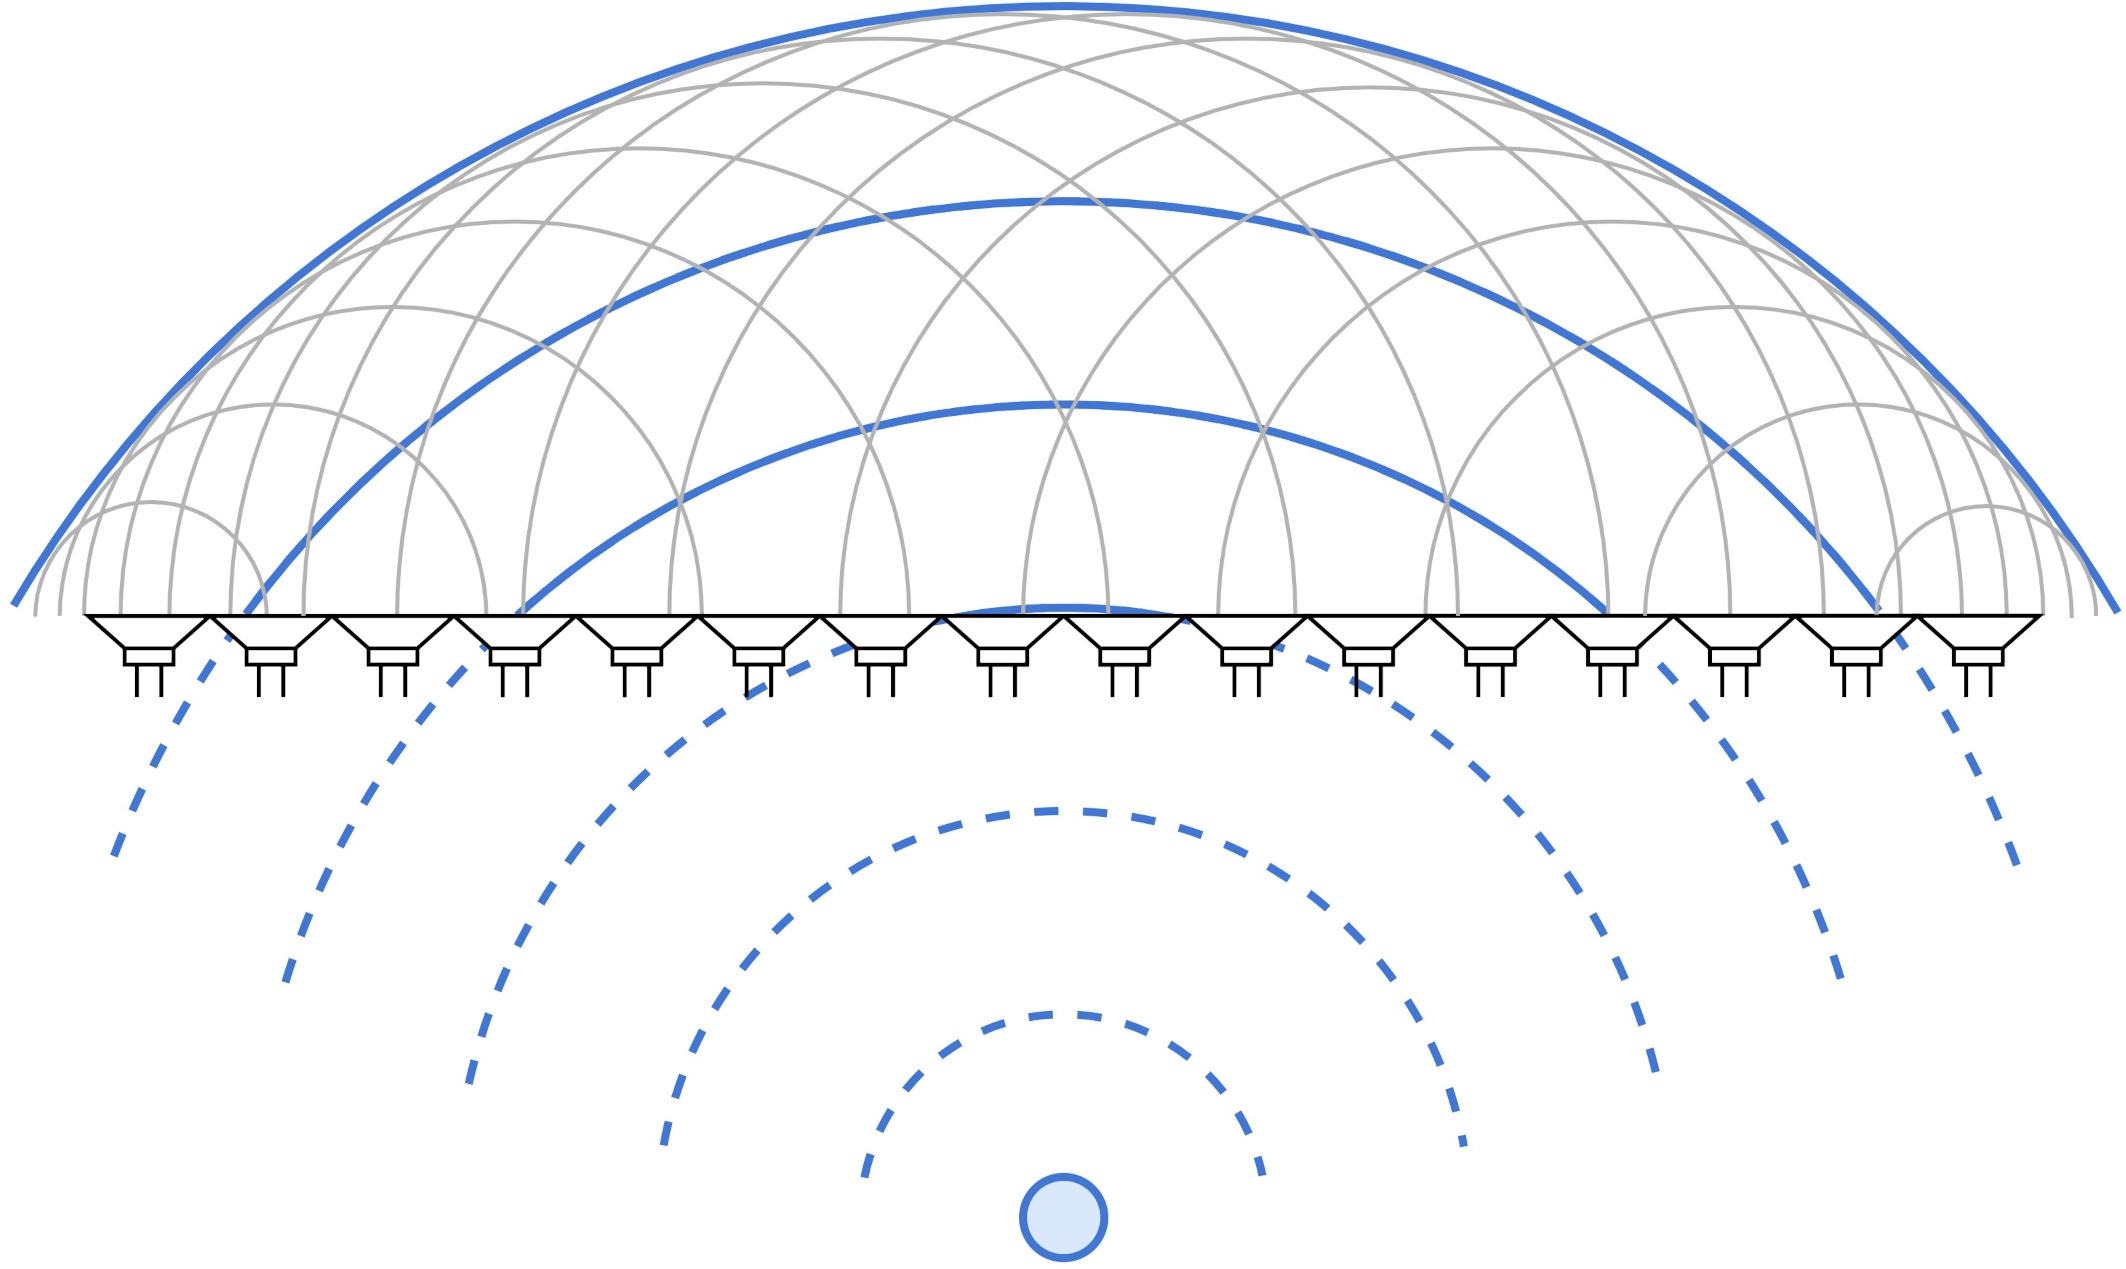
\includegraphics[width=.75\textwidth]{figures/wfs_1}
        \caption{\textit{Holophony}.
        Huygens' principle states that the propagation of a wavefront
        can be recreated by a collection of secondary point sources.
        The bottom of the figure represents a virtual sound field, and the top a
        real sound field, separated by a row of secondary point sources
            (loudspeakers).
            The small circle represents a virtual sound source and the dashed arcs
            are virtual wavefronts associated with that sound source;
            the small solid arcs are wavefronts produced by the array of secondary
            point sources;
            the large solid arcs represent the propagation of a reconstructed
            wavefront in the real sound field.}
        \label{fig:wfs_1}
    \end{figure}

    Physical approaches fall into two main types: wave field synthesis
    (WFS)~\citep{berkhout_acoustic_1993} and
    ambisonics (and higher-order ambisonics \textemdash{}
    HOA)~\citep{frank_producing_2015}.
    Rather than directly manipulating sound localisation cues, these types seek to
    trigger those cues indirectly by synthesising a sound field as if it had been
    created by `true' acoustic sources.

    In the case of ambisonics, the sound field is decomposed into `spherical
    harmonics', spatial functions described by linear sums of directional
    components of increasing order~\citep{nicol_sound_2017}.
    Like periphonic approaches, ambisonics suffers from a sweet-spot effect
    which worsens with attempts to reproduce sounds of higher frequency, but can
    be mitigated (at greater computational expense) by reproducing higher-order
    modes and increasing the density of the distribution of secondary sources.

    Wave Field Synthesis is based upon Huygens' principle, originating in the
    field of optics, which states that a propagating wavefront can be recreated
    by a distribution of secondary point sources~\citep{mueller_acoustic_1971,
        berkhout_acoustic_1993,belloch_performance_2021} (see
    \figref{fig:wfs_1}).
    WFS is variously termed a form of \textit{acoustic holography} or
    \textit{holophony}~\citep{berkhout_holographic_1988,ahrens_analytic_2012}.
    Effectively, by timing the reproduction of an input signal at an array of
    secondary sources, a wavefront associated with a virtual sound source can be
    synthesised.
    To simulate auditory cues related to perceived distance, a filter can be
    applied to model losses to the virtual medium of acoustic propagation.
    The principle assumes a continuous array of secondary sources but of course
    in practice it is necessary to use a discrete array of loudspeakers, which,
    much as is the case with HOA, has consequences for spatial resolution;
    to mitigate the issue of spatial aliasing, whereby sounds of higher
    frequency cannot be recreated unambiguously~\citep{winter_geometric_2018},
    secondary sources should be placed very close together.
    Consequently, to serve a large listening area, many speakers, and thus many
    audio channels, are required.

    Via appropriate timing of the delivery of a primary sound source to the
    secondary source array, it is possible to synthesise virtual sound sources,
    plane waves, and \textit{focused} sound sources, corresponding with concave,
    flat, and convex synthesised wavefronts respectively; the latter, dependent
    on the location of the listener, appear to emanate from within the real
    sound field, rather than its virtual counterpart.

    \begin{figure}[ht]
        \centering
        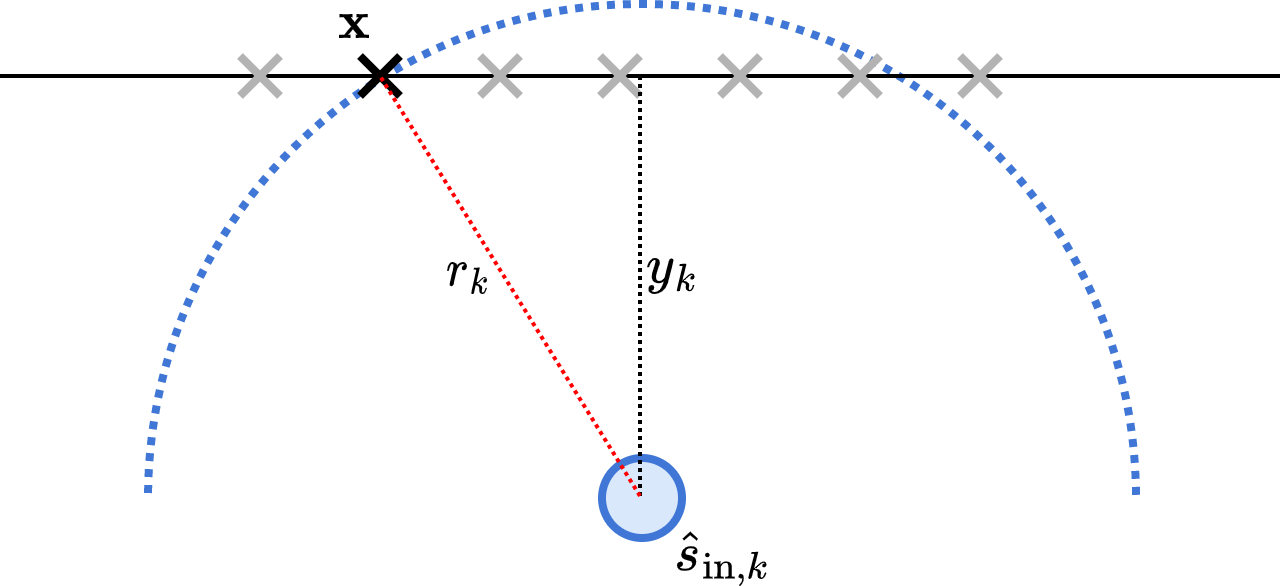
\includegraphics[width=.75\textwidth]{figures/wfs_2}
        \caption{
            The driving signal for the WFS secondary source at position $\bfx$,
            for virtual primary source $\sigink$, is dependent on the distance
            $r_k$ of the primary source from the secondary source.
            This corresponds with a propagation delay via the simulated medium of
            propagation, coupled with a filter describing losses to that medium.
        }
        \label{fig:wfs_2}
    \end{figure}

    Focusing on the former kind, however, for $m$ virtual sources, the time-domain
    driving signal $\hat{d}$ for the secondary source at $\bfx$ may be expressed
    as:
    \begin{equation}
        \label{eq:driving-signal}
        \hat{d}(\bfx,t) = \sum_{k=0}^{m-1}\sigink \ast d_k(\bfx,t),
    \end{equation}
    where the driving function $d_k$ is~\citep{ahrens_analytic_2012}:
    \begin{equation}
        \label{eq:driving-function}
        d_k(\bfx,t) = \frac{y_k}{r_k}f(t) \ast \delta\left(t - \frac{r_k}{c}\right).
    \end{equation}
    The \textit{WFS prefilter} $f(t)$ is a function that simulates the absorption of
    energy into the simulated medium of acoustic propagation.
    The delta function $\delta$ has the effect of delaying the prefilter, and thus
    $\sigink$, by the time of propagation for a medium with propagation speed $c$
    (typically modelled as \qty[per-mode=symbol]{343}{\m\per\s} for sound in air).
    The components of the driving function are depicted in \figref{fig:wfs_2}.

    \subsubsection{State of the Art Spatial Audio Installations}
    \label{subsubsec:spatial-sota}

    As described, for optimal spatial resolution, systems implementing ambisonics
    and WFS require many output channels; in effect, the more channels, and the
    greater the loudspeaker-density, the better.

    The Multisensory Experience Lab at Aalborg University (AAU), Copenhagen, hosts
    a 64-channel, square-array WFS system covering an area of
    \qtyproduct{4 x 4}{\m}~\citep{grani_gestural_2016}.
    It is driven by a Mac Pro desktop computer, connected, via a USB MADI
    (Multichannel Audio Digital Interface) interface, to two 32-channel MADI to
    analogue converters.
    Though this system's WFS engine is provided by open-source \textit{WFSCollider}
    software,\footnote{\url{https://github.com/GameOfLife/WFSCollider}} being a
    centralised system, the computer that co-ordinates its operation is powerful
    \textemdash{} 12-core CPU, \qty{64}{\giga\byte} RAM \textemdash{} and was costly
    at the time of purchase; likely on the order of several thousand Euros.
    With further regard to cost, the current equivalent MADI to analogue converter
    models are priced at roughly \texteuro{5000} apiece.
    Excluding the cost of loudspeakers (and the gantry upon which they are mounted)
    one may reasonably place an estimate of \texteuro{250} per output channel on
    this system.

    The world's largest dedicated WFS system, at TU Berlin, features over 800
    output channels served by a distributed cluster of fifteen computers acting
    as audio nodes and two additional control
    computers~\citep{baalman_renewed_2007}.\footnote{
        See also
        \url{https://tu.berlin/en/ak/research/projects/wellenfeldsynthese-fuer-einen-grossen-hoersaal}
        and WFS speaker module produced by Four Audio for installation at TU
        \url{https://four-audio.com/en/products/wfs/}.
    }
    The fifteen audio nodes of the TU Berlin system are each equipped with a MADI
    audio interface, connected to a MADI to ADAT bridge;
    these can, at the time of writing, be purchased for around
    \texteuro{\num{1400}} and \texteuro{\num{4500}} each, respectively, for a
    total of \texteuro{\num{88500}}.
    Imagining \texteuro{2000} per computer, a conservative estimate of
    \texteuro{150}/channel may be reached, however the expense associated with
    this  system is difficult to assess as it is tied to the concert hall space
    in which it resides.
    Indeed, one thing besides expense that unites the systems at AAU and TU
    Berlin, plus similar installations at IRCAM (Paris)\footnote{
        \url{https://www.ircam.fr/article/connaissez-vous-lespace-de-projection}
    }
    and the 512-channel system at the Rensselaer Polytechnic Institute
    (NY, USA)\footnote{
        \url{https://empac.rpi.edu/about/building/venues}
    } is their \textit{in-situ} nature;
    these are site-specific systems with, at best, limited flexibility.

    What one is afforded by WFS installations of this scale and expense, however, is
    high quality audio reproduction with tantamount to perfect output synchronicity;
    the integrity of the holophonic effect of WFS is, unavoidable matters of spatial
    aliasing aside, guaranteed.

    \subsection{Distributed Audio Systems}\label{subsec:distributed-audio-systems}

    As alluded to earlier in this section, our aim is to distribute the problem
    of audio spatialisation, and it is worthwhile to revisit why this is the
    case.
    In the broadest terms, a distributed system is \textit{``a collection of
    independent entities that cooperate to solve a problem that cannot be
    individually solved''}~\citep{kshemkalyani_distributed_2011}.
    An ideal distributed system is characterised by: \textit{modularity}, being
    comprised of separate, interchangeable entities; \textit{scalability}, being
    extensible without incurring a performance penalty to the system as a whole,
    and; \textit{improved performance/cost ratio}, since it can be constructed
    to meet the proportion that circumstances require, with the minimum degree
    of redundancy.
    Additionally, for algorithms that can be effectively \textit{parallelised},
    a distributed system may provide more aggregate computational power than its
    centralised counterpart.

    Where a distributed system may suffer, by contrast, is in terms of
    reliability.
    Nodes in a distributed computational system must be served with power and
    access to the data they require in order to operate, which entails a
    proliferation of potential points of failure.
    The other side to the coin of modularity is a concern regarding the
    programmability of such a system;
    ensuring that all entities possess up-to-date instructions for operation may
    not be trivial.
    Further, some algorithms may be better suited to parallelisation than
    others; efficient use of an increased computational resources is not
    guaranteed.

    Distributed audio processing is by no means a matter without precedent.
    (Indeed, the WFS installation at TU Berlin described in
    \secref{subsubsec:spatial-sota} is of course a distributed system, albeit
    not an especially accessible one.)
    A selection of prior work in distributed DSP and audio spatialisation, plus
    systems incorporating microcontrollers and single-board computers is
    detailed below.

    \subsubsection{State of the Art Distributed Audio Systems}

    Applications of SoundWIRE to what its creators termed \textit{Internet
    Acoustics}~\citep{chafe_physical_2002} obviously represent a case of
    distributed audio processing.
    These include a network reverberator~\citep{chafe_i_2018}, or
    \textit{``transcontinental echo chamber''}~\citep{chafe_simplified_2000},
    plus the aforementioned \textit{Network Harp}.
    Experiments of this sort were intended initially as sonifications of QoS
    \textemdash{} a characteristic of network systems that is difficult to
    represent in graphical or textual form due to the ephemeral nature of the
    phenomena of jitter and packet loss \textemdash{} but stand as fascinating
    applications in their own right of digital audio in the age of computer
    networking.
    Subsequent work on JackTrip has focused on optimising networked audio less
    as a creative tool in itself, and more in service of the social and communal
    aspects of music participation and appreciation in a networked world, topics
    that came to the fore in computer music research during the
    COVID 19 pandemic~\citep{bosi_experiencing_2021,
        sacchetto_jacktrip-webrtc_2021}.
    That being said, more recent work on Internet Acoustics in an embedded
    context has yielded a port of JackTrip to the Raspberry
    Pi~\citep{chafe_jacktrip_2019}.

    Examples of distributed music production systems include the work of
    Lago and Kon~\citep{lago_middleware_2003}, whose UDP-based system featured
    clients that acted as delegates for audio processing, and Gabrielli et
    al.~\citep{gabrielli_networked_2012}, who demonstrated a wireless relay of
    audio and control-data processors.
    Latency was an important metric for the latter system, and the authors
    measured latency via transmission round-trip times using a sawtooth wave as
    a timer (see \secref{subsec:technical-evaluation} for an application of this
    technique).

    Distributed approaches to audio spatialisation include Lopez-Lezcano's
    ``network sound card''~\citep{lopez-lezcano_jack_2012}, and embedded
    implementations as described by Devonport and
    Foss~\citep{devonport_distribution_2019} and Belloch et
    al.~\citep{belloch_performance_2021}.
    The latter two address aims closely aligned with the work described here,
    but are based on costly computing platforms.
    Devonport and Foss used AVB, and thus PTP, for synchronisation; Belloch et
    al.\ employed a GPU-based hardware platform, reporting client
    synchronisation to the millisecond range \textemdash{} likely not sufficient
    for timing-critical audio spatialisation effects.

    Also of interest is the OTTOsonics
    project~\citep{mitterhuber_ottosonics_2022};
    its emphasis on a fully-costed, flexible, do-it-yourself alternative to
    conventional spatial audio systems is pertinent to this work, though it
    diverges in its use of AVB, and associated hardware for audio transmission.
    A full 24-channel OTTOsonics system, including speakers and audio interface,
    is costed at around \texteuro{2600} (\texteuro{108.33}/channel), however,
    which certainly places it favourably when compared with state-of-the-art
    spatialisation systems.

    \dots [Probably needs a paragraph here to wrap up.]

    \section{Method}\label{sec:method}

    \dots [And/or here, to ease the reader in.]

    Being a system distributed across distinct computing platforms (a general
    purpose computer; a network of microcontrollers), and software elements
    serving a variety of purposes (server and client instances for transmission
    and reception of networked audio and control data, plus a DSP algorithm), it is
    important to consider each of these elements in detail.
    In the subsections that follow, these elements are described;
    finally an overview of the devised system is provided.

    \subsection{The Networked Audio Server}\label{subsec:the-networked-audio-server}

    TCP is, as described in \secref{subsubsec:protocols-systems}, a
    connection-based, one-to-one protocol, so the JackTrip connection model enforces
    a sort of pseudo-connectionfulness on the otherwise connectionless UDP.\
    The result is a system which permits only unicast UDP transmission, and, for
    multiple clients, must send a duplicate of the outgoing stream of audio
    datagrams to each connected client.
    A JackTrip server creates a sender and a receiver task for each client that
    connects~\citep{caceres_jacktrip_2010};
    notionally this entails, should enough clients connect, exhaustion of all
    available network bandwidth;
    as such, a unicast system does not meet the requirement of scalability as
    described in \secref{subsec:distributed-audio-systems}.

    A multicast NetJACK server was considered, but creating a client
    implementation on what is essentially a bare-metal platform in the shape of
    the Teensy, was not practical.
    Further, due to a break in compatibility with Mac OS X systems, JACK-based
    approaches are not truly cross-platform.\footnote{
        A successor to the defunct CoreAudio/JACK bridge has been proposed but
        remains unrealised:
        \url{https://github.com/jackaudio/jack-router/blob/main/macOS/docs/JackRouter-AudioServerPlugin.md}.
        This issue of course also affects the viability of the JackTrip-based
        approach.
    }
    Prioritising simplicity, in the form of an audio server with minimal
    dependencies and a very specific task to achieve, we embarked upon the
    design of a bespoke multicast networked audio server.

    \subsubsection{Designing a Networked Audio Protocol}\label{subsubsec:designing-a-protocol}

    Dependent on the intended application, and if assumptions can be made about
    matters such as sampling rate and bit resolution, a \textit{no-protocol}
    approach, such as described by
    Lopez-Lezcano~\citep{lopez-lezcano_jack_2012}, may be a viable one.
    To improve the flexibility of the system and render it somewhat
    future-proof, however, a simple packet header was devised.
    Its structure is given in \lstref{listing:packet-header}.

    \begin{codelisting}{
        Packet header structure,
        label=listing:packet-header,
        minted language=cpp,
        minted style=xcode,
        float=ht
    }
        struct PacketHeader {
            uint16_t SeqNumber;
            uint8_t BufferSize;
            uint8_t SamplingRate;
            uint8_t BitResolution;
            uint8_t NumChannels;
        };
    \end{codelisting}

    The resulting six-byte header comprises a two-byte (unsigned 16-bit integer)
    packet sequence number, to be incremented by the sender, plus four further bytes
    describing the structure of the audio data in the packet.
    Commonly-encountered sampling rates, and buffer sizes greater than 255, cannot
    be represented by unsigned eight-bit integers, so these are supported by
    enumerations inspired by those used by JackTrip.\footnote{
        \url{https://github.com/jacktrip/jacktrip/blob/v1.6.8/src/AudioInterface.h\#L56}
    }

    \texttt{BufferSize} describes the number of audio frames per packet\footnote{
        Often used interchangeably with the word \textit{sample}, a \textit{frame}
        represents the samples for all channels for a given sample instant;
        thus the number of frames in a network packet or audio buffer is the number
        of samples divided by the number of channels.
    } as the $n$th power of 2; for example, the enumeration \texttt{BufferSizeT}
    features a member \texttt{BufferSizeT::BUF16}; 16 being the fourth power of 2,
    this member is assigned the number 4.
    The \texttt{BitResolution} field could be used to transmit one of 8, 16, 24, or
    32 as-is; there is a utility, however, when decoding a packet, in knowing the
    number of \textit{bytes} per audio sample, so this is the number that is
    represented, e.g. \texttt{BitResolutionT::BIT16} takes the value 2, the number
    of bytes in a 16-bit integer.

    For well-formed packets, \texttt{BufferSize} could be inferred from the size of
    the packet (minus its header), divided by \texttt{NumChannels} and
    \texttt{BitResolution}.
    To permit scope for the detection of malformed packets, however, the expense
    of an additional byte in the header was deemed a reasonable one.
    Finally, the sequence number is intended as a means for a recipient to identify
    the occurrence of packet loss, and will wrap around to zero every \num{65536}
    packets.

    One piece of information that is not stated in the packet header is the manner
    in which audio samples in the packet should be interleaved.
    The assumption taken \textemdash{} indeed, the same assumption used by JackTrip
    \textemdash{} is that audio data is channel-interleaved, i.e.\ audio data
    consists of a contiguous block of samples for one channel, followed by a block
    for the next channel, and so on.

    \subsubsection{Server Design}

    \begin{figure}[ht]
        \centering
        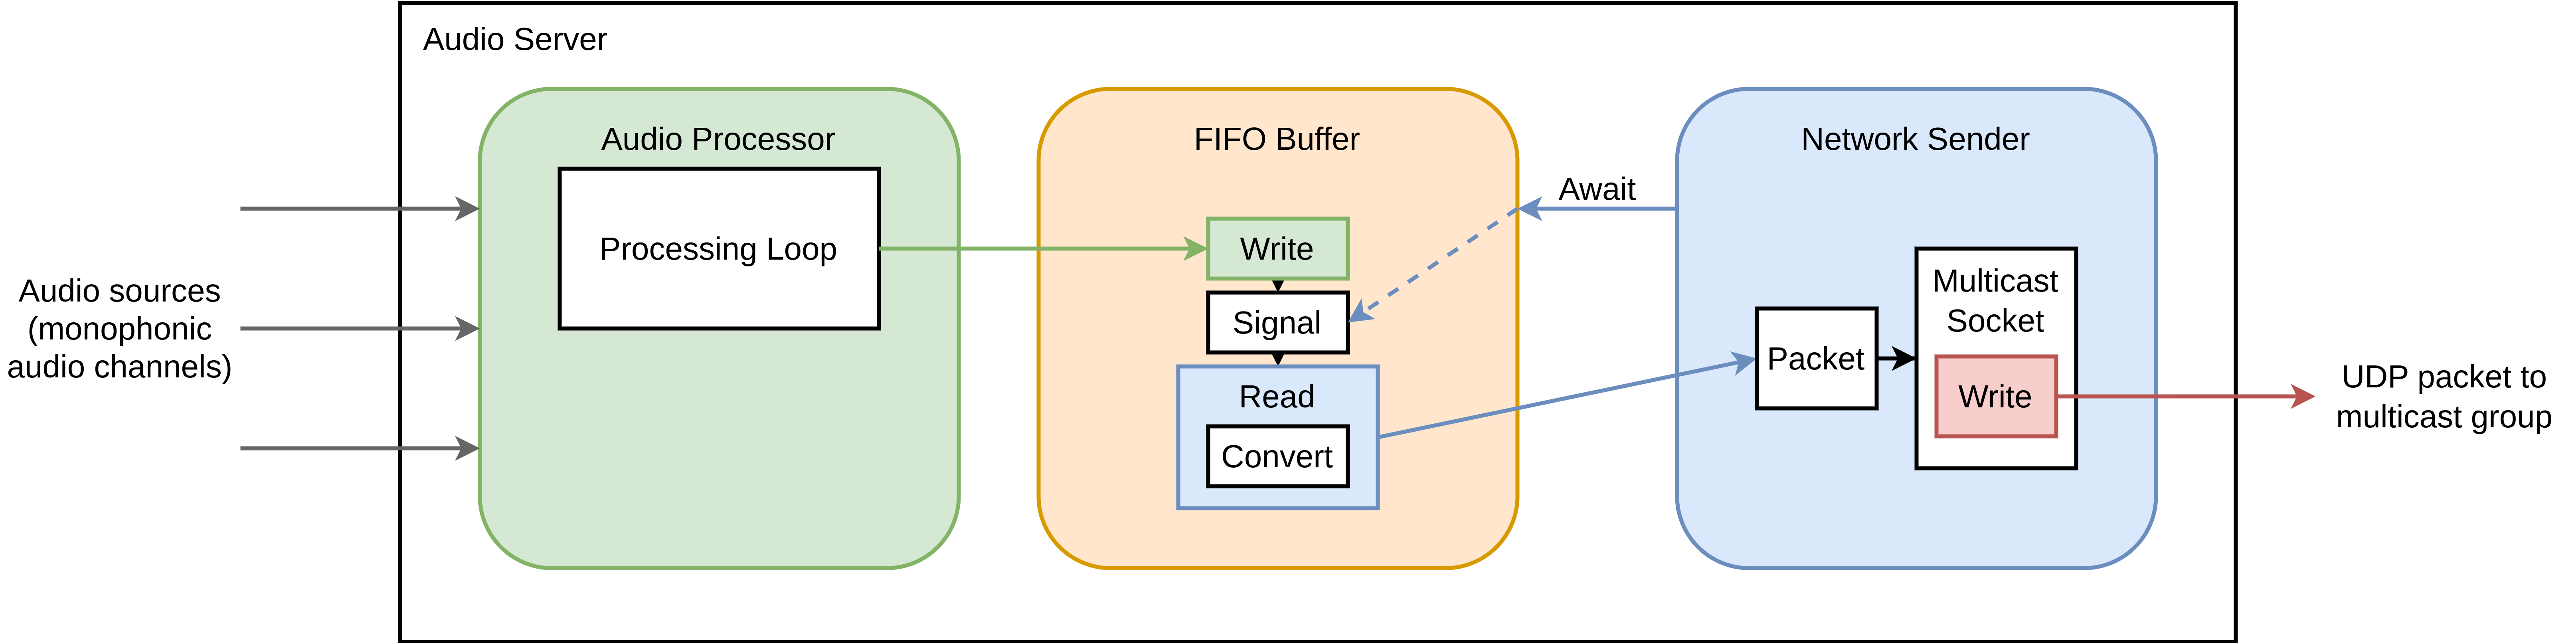
\includegraphics[width=\textwidth]{figures/audio-server}
        \caption{Overview of operation of the networked audio server.
        The network sender awaits notification of readiness to read samples from a
        first-in-first-out buffer of audio samples.
        The audio processor receives audio channels from a multichannel source
            (e.g. a DAW); at each iteration of its processing loop, it writes
            samples to the FIFO; upon write-completion, the FIFO sends a signal to
            the network sender that a block of samples is ready.
            Samples are converted to the desired bit resolution and byte order and
            bundled into a UDP packet which is then written to the network.}
        \label{fig:audio-server}
    \end{figure}

    The networked audio server was written in C++ using utility classes provided
    by the JUCE framework for the development of audio applications\footnote{
        JUCE 7.0.5 \url{https://github.com/juce-framework/JUCE}
    }
    and is encapsulated as a class called \texttt{NetAudioServer}.
    Initial development was conducted on a basic console application, and later
    work targeted a DAW plugin comprising a consolidated audio server and wave
    field synthesis controller.

    The \texttt{NetAudioServer} instance expects to receive blocks of
    multichannel audio from an audio application's main processing loop.
    It sets up network \textit{sender} and \textit{receiver} execution threads, and
    assigns a network socket to each; a socket is essentially a numerical identifier
    for an
    \textit{``endpoint for [network] communication''}~\citep{kerrisk_socket2_2023}
    to which a type \textemdash{} \texttt{SOCK\_STREAM} for TCP on
    \texttt{SOCK\_DGRAM} for UDP \textemdash{} can be assigned.
    To avoid potentially blocking the audio application's main processing thread
    with networking operations, upon receiving an audio block the server writes it
    to an intermediate buffer \textemdash{} a first-in-first-out (FIFO) structure
    \textemdash{} and signals the sender thread that a block is ready for
    transmission.
    The sender thread, which as been awaiting such a signal, then requests samples
    from the FIFO; these are stored as contiguous channels of 32-bit floating point
    samples and converted, when requested, to the bit resolution specified in a
    packet header created when \texttt{NetAudioServer} is initialised.
    Byte order, or \textit{endianness}~\citep{cohen_holy_1981}, is also specified as
    part of this conversion.
    Though network byte order is typically big-endian, or Most Significant Byte
    (MSB) first, it was found that little-endian transmission meant that samples
    could be decoded trivially at the client side.\footnote{
        Endianness is a thorny issue \textemdash{} just consider Danny Cohen's
        \textit{...Plea for Peace}~\citep{cohen_holy_1981}.
        To appeal momentarily to authority, JackTrip too transmits audio data (and
        port numbers, etc.) little-endian, ``network byte order'' notwithstanding.
    }
    Upon receiving the requested samples, the sender thread writes these to its
    socket, which has been configured to connect to a UDP multicast group.
    This process is illustrated in \figref{fig:audio-server}.

    \begin{codelisting}{
        Network capture: ethernet frame containing a UDP audio packet,
        label=listing:audio-packet,
        minted language=text,
        float=ht
    }
       00 01 02 03 04 05 06 07  08 09 0a 0b 0c 0d 0e 0f

0000   01 00 5e 04 e0 04 a0 36  bc d0 aa 18 08 00 45 00   ..^....6......E.
0010   00 62 8b b5 40 00 01 11  63 1a c0 a8 0a 0a e0 04   .b..@...c.......
0020   e0 04 39 f9 a3 56 00 4e  66 2b df 1c 04 02 02 02   ..9..V.Nf+......
0030   3f 7a 40 7a 41 7a 42 7a  43 7a 44 7a 45 7a 46 7a   ?z@zAzBzCzDzEzFz
0040   47 7a 48 7a 49 7a 4a 7a  4b 7a 4c 7a 4d 7a 4e 7a   GzHzIzJzKzLzMzNz
0050   2c 8c ff 88 43 86 05 84  46 82 00 81 44 80 00 80   ,...C...F...D...
0060   45 80 ff 80 46 82 06 84  41 86 02 89 29 8c db 8f   E...F...A...)...
    \end{codelisting}

    \lstref{listing:audio-packet} shows an example network capture of an outgoing
    audio packet.
    Bytes \texttt{0x0000} to \texttt{0x0029} comprise the headers for the data link
    (ethernet), network (IPv4), and transport (UDP) OSI layers including the
    destination address: at position \texttt{0x001e}, the bytes \texttt{0xe004e004},
    or \texttt{224.4.224.4}, a valid (and unassigned) UDP multicast address from the
    second ad-hoc address block as specified in the IANA multicast address
    assignment guidelines~\citep{meyer_iana_2010}.
    The six subsequent bytes are the header inserted into the packet by
    \texttt{NetAudioServer}.
    In \lstref{listing:audio-packet} these are:
    \begin{itemize}
        \item~\texttt{0x1cdf}: a sequence number (little-endian) of
        \numDec{7391};\footnote{Subscript 10 is employed here to indicate a decimal
        number.}
        \item~\texttt{0x04}: buffer size \num{4} corresponding with
        \texttt{BufferSizeT::BUF16};
        \item~\texttt{0x02}: sampling rate \num{2} corresponding with
        \texttt{SamplingRateT::SR44};
        \item~\texttt{0x02}: bit resolution \num{2} corresponding with
        \texttt{BitResolutionT::BIT16};
        \item~\texttt{0x02}: \num{2} audio channels.
    \end{itemize}

    Audio data begins at byte \texttt{0x0030}.
    Since the header indicates that there are two channels of 16-bit audio, and a
    buffer size of 16 frames, it is clear that the data for channel 1 encompasses
    the 32 bytes from \texttt{0x0030} to \texttt{0x004f}, and channel 2 the
    remaining bytes.

    Here, channel 1 is a test signal, a unit amplitude-increment unipolar sawtooth
    wave, i.e.\ a signal whose amplitude starts at zero, and increments by 1 at each
    sample until it reaches the maximum value that a signed 16-bit integer may take
    \textemdash{} \numDec{32767} \textemdash{} at which point it wraps around to
    zero and repeats.
    This test signal serves two important purposes.
    First, its impulse-like behaviour once every \num{32768} samples (roughly
    \qty{.74}{\s} at a sampling rate of \qty{44.1}{\kHz}) is useful for taking basic
    synchronicity measurements, e.g.\ involving connecting two clients' audio
    outputs to an oscilloscope.
    Second, this numerically-predictable signal serves as a means to inspect the
    integrity of the audio server algorithm, and to verify that the expected
    sample interleaving and endianness is employed.
    Inspecting the first sixteen samples of the first audio channel
    it is evident that the amplitude values increment on a per-sample basis, and,
    since it is the first byte that increases with each sample, that samples are
    transmitted little-endian.

    The purpose of the server's receiver thread is to poll its socket for traffic
    reaching the multicast group from connected clients.
    Clients are programmed to return a stream of packets of audio data to the
    multicast group, and the receive thread uses the existence of a such a stream,
    with a given origin IP address, to indicate the presence of a client at that
    address.
    If a client fails to return a packet for more than \qty{1}{\second} it is
    considered disconnected.
    Clients could announce their presence with any periodic UDP transmission, but
    the possibility of returning audio data facilitates the measurement of client
    synchronicity via transmission round trip times (see
    \secref{subsec:technical-evaluation}).

    \subsubsection{Transmission Considerations}\label{subsubsec:transmission-considerations}

    Ethernet frames, and UDP datagrams by extension, are subject to size
    limitations.
    The maximum transmissible unit (MTU) of a transport medium is the limit on the
    size of a packet that can be sent without fragmentation, i.e.\ without being
    split into multiple sub-packets.
    Two bytes are allocated to the `Total Length' field of the IPv4 header, which
    suggests an MTU of $2^{16}-1=~$\num{65535} bytes;
    in practice, however, the data link layer imposes a basic limit of \num{1500}
    bytes on the payload of an ethernet
    frame~\citep{schiavoni_alternatives_2013,ieee_ieee_2018}.

    With the headers for the data link (Ethernet), network (IPv4), and transport
    (UDP) layers accounted for, plus the audio header described above, in principle
    \num{1452} bytes remain in each packet for audio data.
    Assuming 16-bit resolution, and the transmission of one UDP packet per audio
    buffer, data for up to 90 audio channels can be transmitted at a buffer size of
    16 frames without fragmentation, or up to 45 channels at 32 frames.

    \subsection{The Networked Audio Client}\label{subsec:networked-audio-client}

    \begin{figure}[ht]
        \centering
        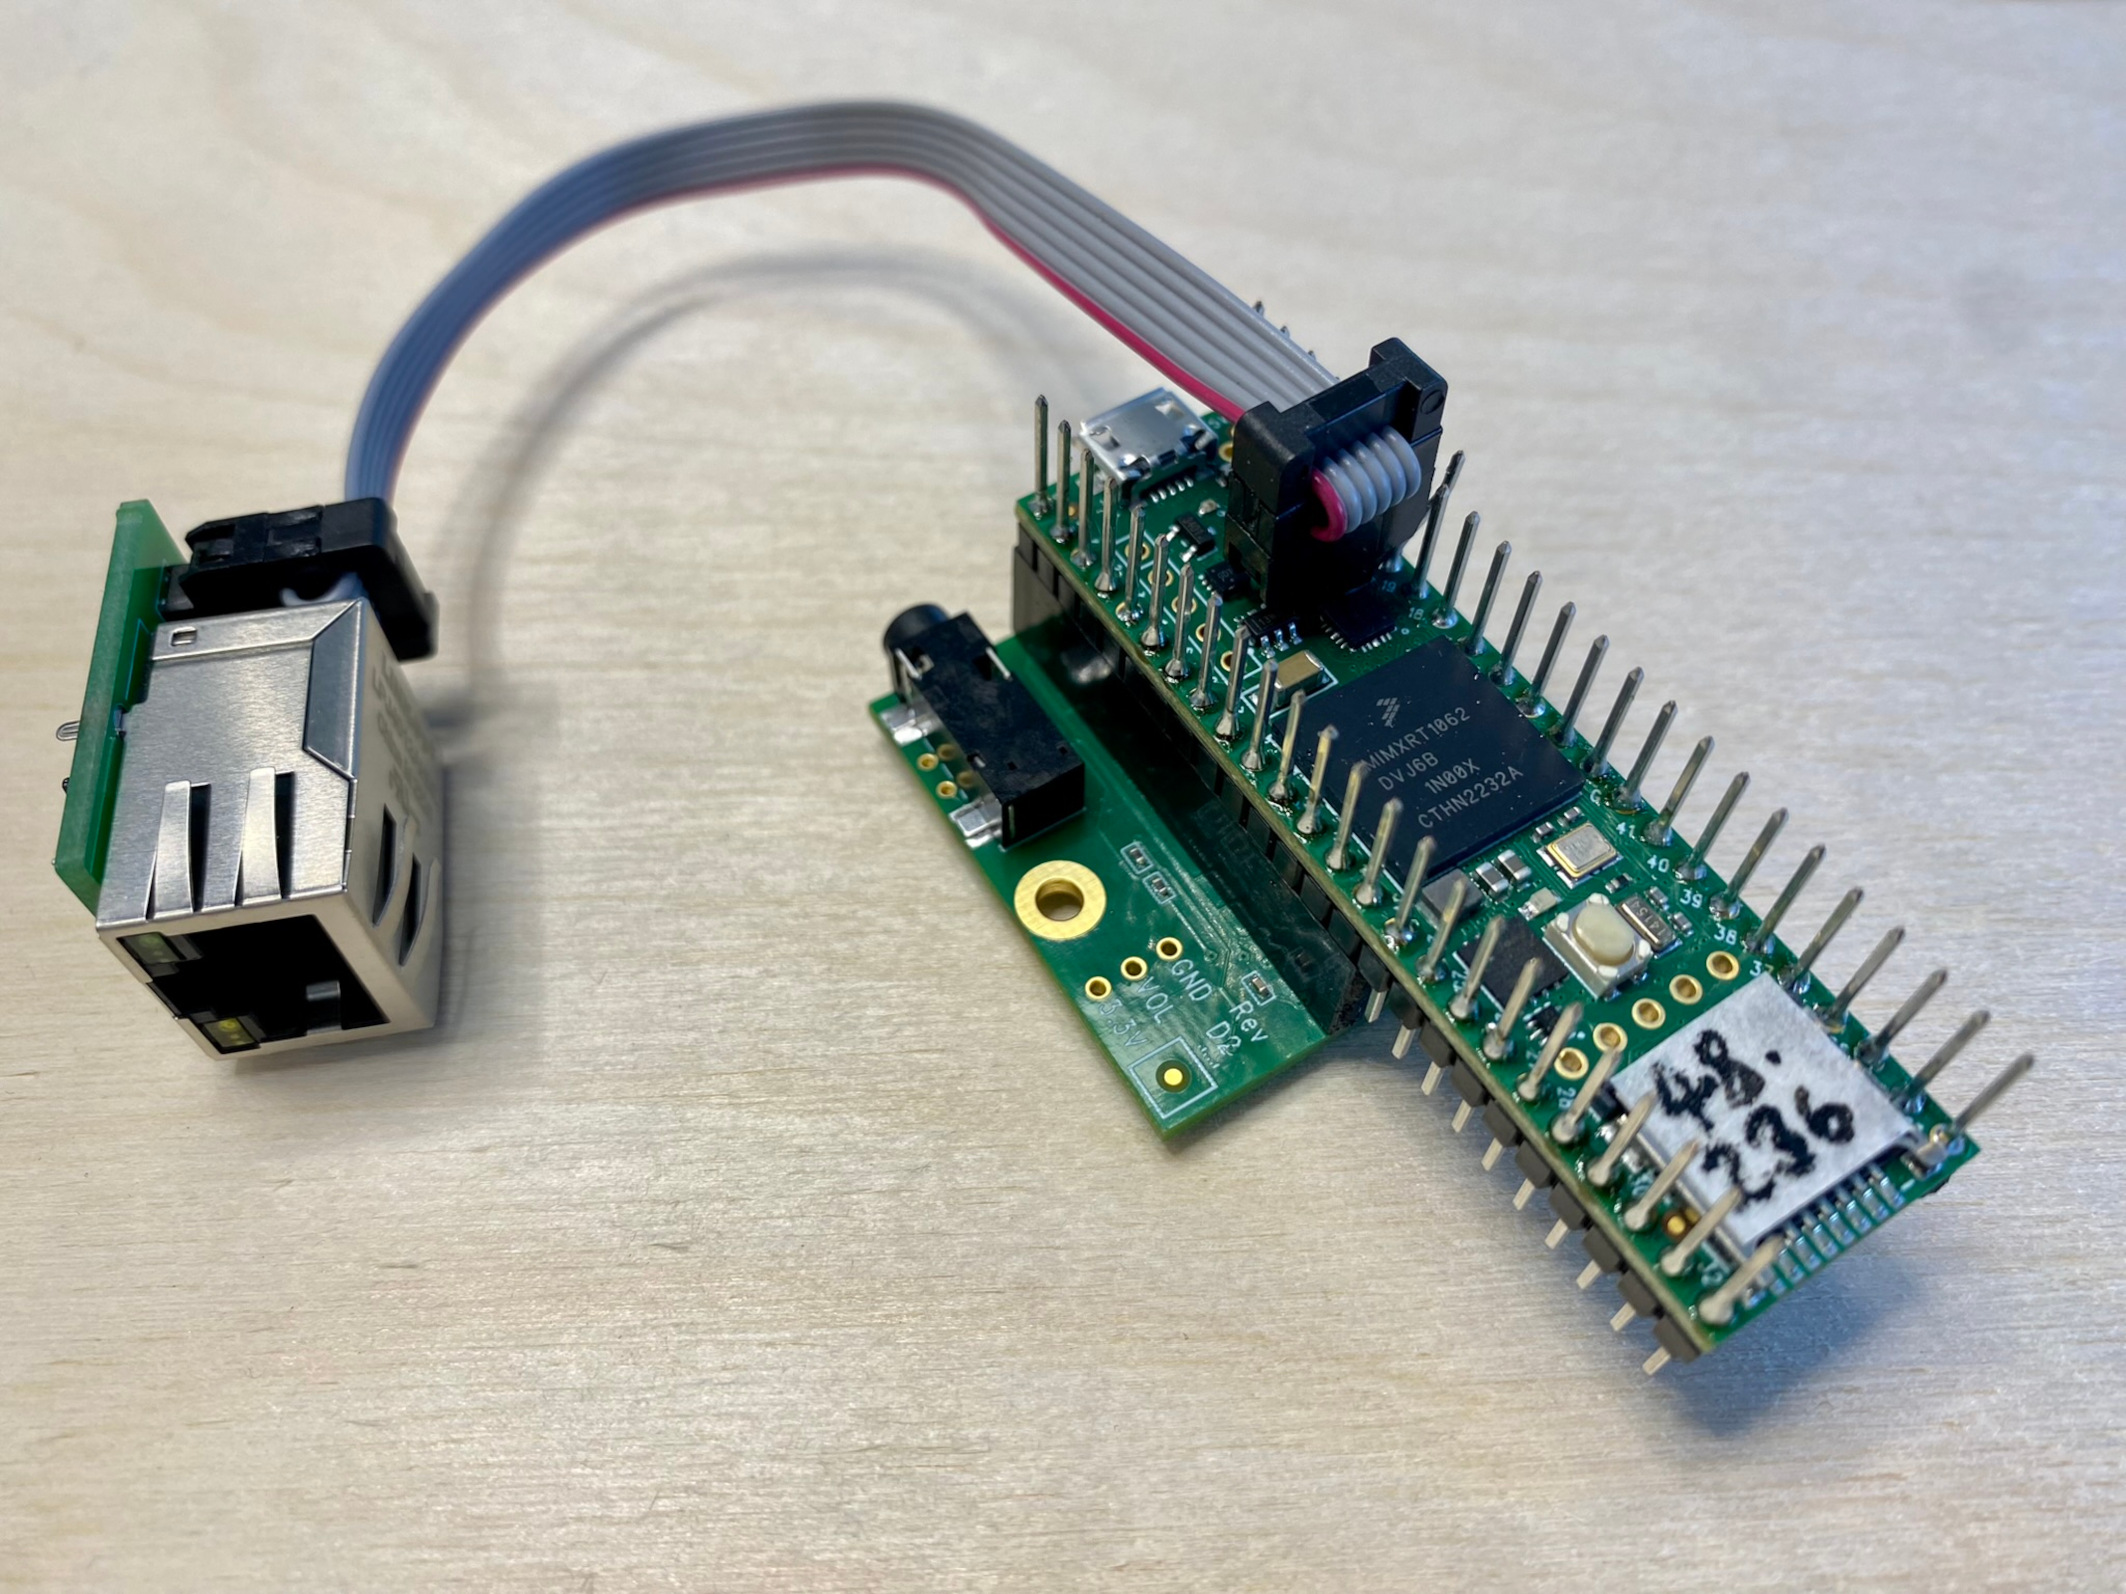
\includegraphics[width=.75\textwidth]{figures/module}
        \caption{A hardware module consisting of Teensy 4.1 microcontroller
            (labelled with the last two bytes of its serial number-derived IP address),
            connected via headers to an audio shield and via ribbon cable to an
            ethernet shield.}
        \label{fig:teensy}
    \end{figure}

    Unlike the networked audio server, which runs on a general purpose computer and
    has access to threads of execution, which it can use to conduct related but
    separate tasks that rely on some central resource (the FIFO buffer alluded to
    above), the client implementation is designed to operate on a microcontroller
    platform that has no operating system, and no native notion of threads.\footnote{
        There is in fact a non-core library, \textit{TeensyThreads}, that provides
        thread-like functionality. It was experimented with during development,
        but found to be incompatible with the interrupt-driven nature of the
        Teensy audio and networking libraries.
    }

    The task of the clients is threefold in nature:
    \begin{enumerate}
        \item~to retrieve packets of audio data from the UDP multicast group;
        \item~to send a stream of audio data back to the multicast group, primarily
        to announce their connectivity;
        \item~to maintain, as far as possible, synchronous operation with the
        server, and (by extension) each other.
    \end{enumerate}

    To address the first two requirements, the client sets up a socket, which it
    uses to both read from and write to the UDP multicast group.

    The client was created as a C++ class named \texttt{NetJUCEClient}, an
    implementation of the Teensy Audio Library class \texttt{AudioStream}.
    \texttt{AudioStream} descendents must implement a method named
    \texttt{update()}; this method is called at each audio hardware interrupt, and
    is where an audio library class should perform operations on the current
    audio buffer.
    Networking operations are conducted from the method
    \texttt{NetJUCEClient::loop}.\
    Avoiding conflicts with audio functionality, this method is called from Teensy's
    top level \texttt{loop()} function.
    A valid Teensy program must define a function by this name, and it is called
    repeatedly from the body of a non-terminating \texttt{while} loop throughout
    operation.

    \begin{figure}[ht]
        \centering
        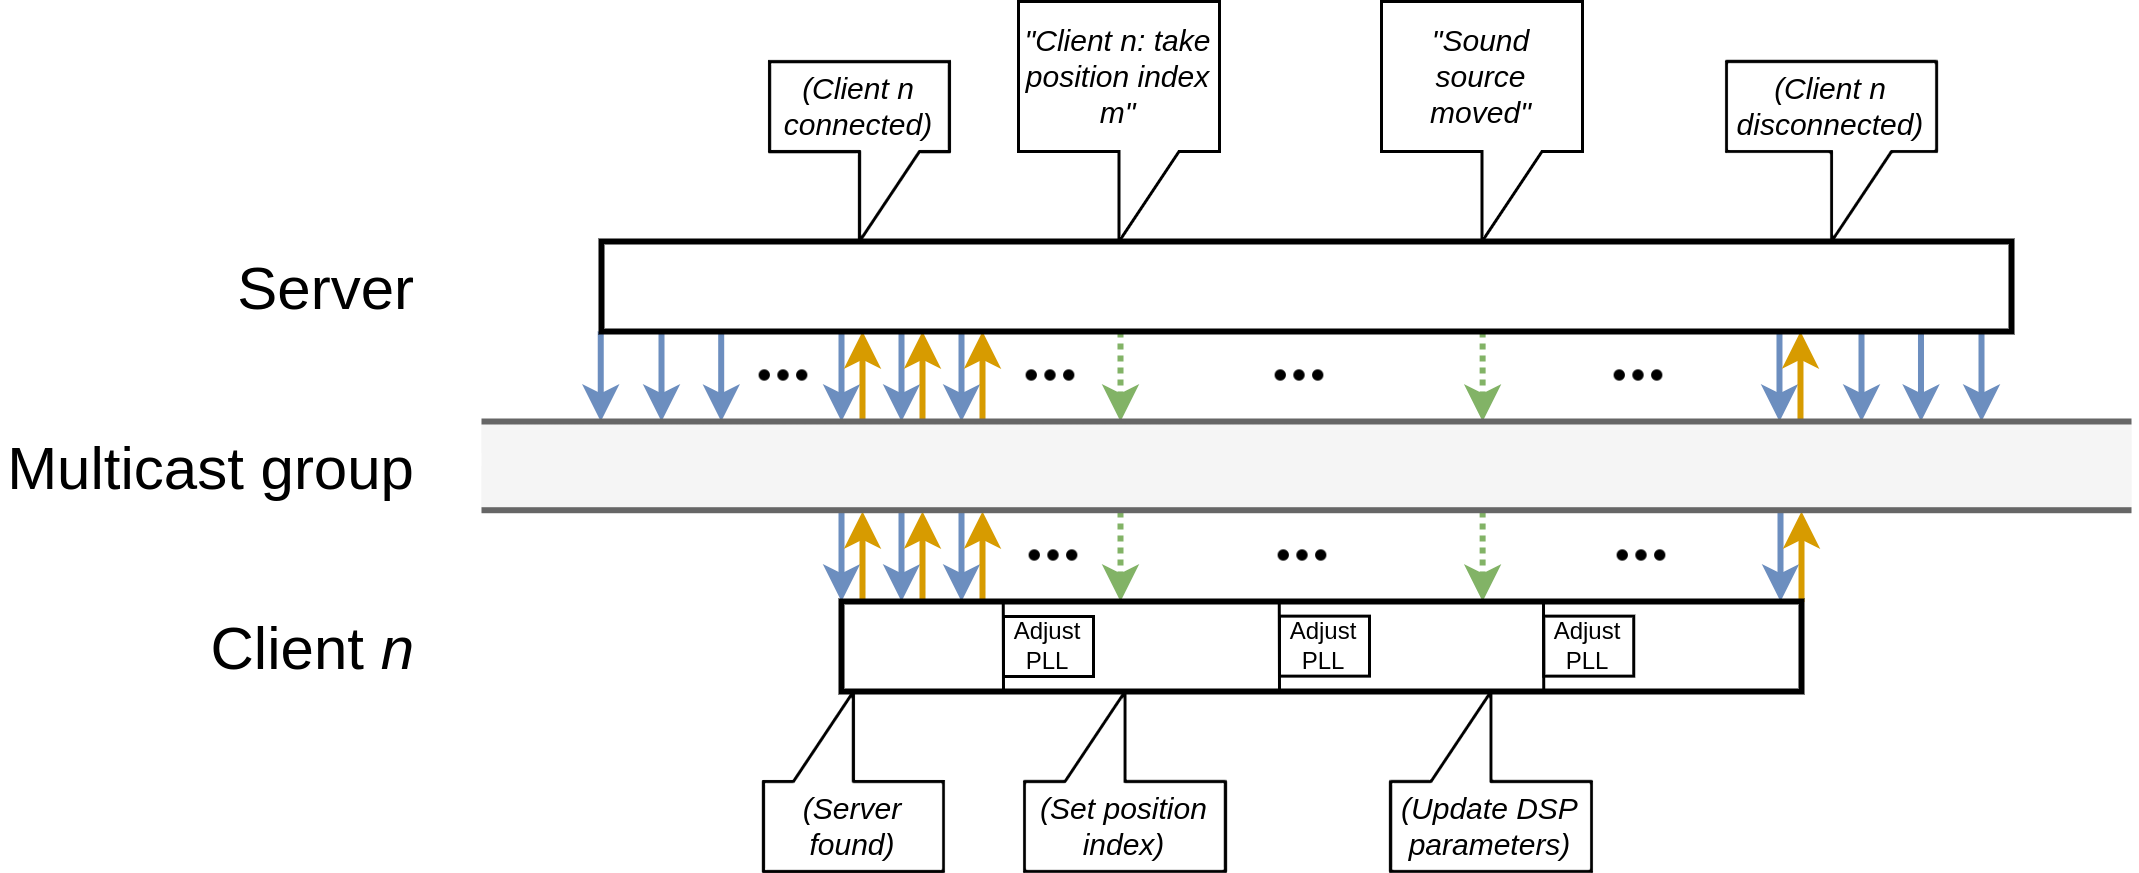
\includegraphics[width=\textwidth]{figures/timeline}
        \caption{
            Example timeline of interaction between the server and a client, via the
            UDP multicast group.
            Solid arrows indicate audio data being sent from the server to the
            multicast group;
            arrows with open heads indicate audio data being sent from the
            client back to the multicast group;
            arrows with dotted tails represent control data.
            Note that the server transmits to the multicast group irrespective of
            the presence of any client.
        }
        \label{fig:timeline}
    \end{figure}

    \begin{codelisting}{
        \texttt{loop} method of the networked audio client implementation,
        minted style=xcode,
        minted language=cpp,
        label=ls:njc-loop,
        float=h
    }
        void NetJUCEClient::loop() {
            receive();

            checkConnectivity();

            send();

            adjustClock();
        }
    \end{codelisting}

    The two sets of operations are linked by way of an intermediate buffer, similar
    to the FIFO employed by the server.
    The client attempts to receive packets from, and, if it has generated a packet's
    worth of audio data, send a packet to, the multicast group on each call to
    \texttt{loop()}, with audio samples from incoming packets written to the
    intermediate buffer (see \lstref{ls:njc-loop}).
    The client also performs a periodic check for the presence of the server, and,
    as described in \secref{subsubsec:client-sync}, makes adjustments to its audio
    clock.
    When multiple clients are present, there are consequently multiple streams of
    audio packets reaching the multicast group.
    To avoid ambiguity and unnecessary packet reads at the client side, server and
    clients transmit audio data to the group on differing port numbers.

    \begin{codelisting}{
        \texttt{update} method of the networked audio client implementation,
        minted style=xcode,
        minted language=cpp,
        label=ls:njc-update,
        float=h!
    }
        void NetJUCEClient::update() {
            doAudioOutput();

            handleAudioInput();
        }
    \end{codelisting}

    On each audio interrupt, the client reads from the intermediate buffer to
    produce samples for audio output.
    It also takes samples reaching its audio inputs and adds those to a packet to be
    sent to the multicast group at the earliest subsequent call to
    \texttt{NetJUCEClient::loop} (\lstref{ls:njc-update}).
    The client's inputs can receive samples from any Teensy Audio Library object to
    which it has been connected programmatically;
    for round-trip time measurements the client's audio outputs were routed back to
    its inputs.
    A timeline of client-server interaction is illustrated in \figref{fig:timeline}.

    \subsubsection{Synchronicity with the Server}\label{subsubsec:client-sync}

    Due to the influence of clock drift and transmission jitter, and since the
    clients constitute a distributed system, with no direct knowledge of each
    other and no authoritative source of time, their third task posed the
    greatest challenge.
    A two-pronged strategy was developed for addressing server-client and
    inter-client timing discrepancies:

    \textbf{Jitter Compensation:}
    Similar to the approach taken in prior
    work~\citep{rushton_microcontroller-based_2023}, clients monitored their
    intermediate buffer for the difference between its write and read positions,
    using a delay-locked loop to keep this difference within an interval of
    one audio buffer's worth of frames.
    This was achieved by way of setting thresholds for the read-write difference,
    and adjusting the read-position increment if the difference fell beyond those
    thresholds;
    increasing the increment if the difference exceeded the high threshold;
    decreasing it should the difference fall short of the low threshold.
    This in turn entailed employing a fractional read-position, and interpolating
    around it to achieve an appropriate sample value; essentially a form of adaptive
    resampling.
    For this purpose a cubic Lagrange interpolator was used; sample values for the
    interpolator were converted from their 16-bit signed integer representation
    to floating point numbers, interpolation conducted, and the resulting value
    rounded to the nearest integer for output.

    \textbf{Clock Drift Compensation:}
    In the absence of an authoritative source of time, clients were set up to infer
    the difference in rate between their own internal clock and that of the server
    by comparing the rate of packet reception from the network to their internal
    audio interrupt rate.
    This was achieved by taking the ratio, over thirty-second intervals, of
    packets written from the network to the intermediate buffer to blocks read
    from the intermediate buffer for audio output.
    This ratio was then used to calculate appropriate divisors to apply to the
    \qty{24}{\MHz} master clock generated by a crystal oscillator on the Teensy,
    adjusting the audio clock's phase locked loop (PLL) to produce an adjusted audio
    sampling rate.
    The aim of this approach was to minimise reliance on the adaptive resampler
    described above, and ultimately encourage all clients to run at the same audio
    rate as the server.

    \subsection{The Audio Spatialisation Algorithm}\label{subsec:wfs-algorithm}

    WFS was chosen for implementation due to the comparative ease with which the
    WFS algorithm can be parallelised.
    Equations~\eqref{eq:driving-signal} and~\eqref{eq:driving-function} (page
    \pageref{eq:driving-signal}) illustrate that the driving signal for a given
    secondary point source is dependent only on the signals and relative
    positions of the virtual primary sources, and is independent of the driving
    signals for the other secondary sources.

    With some modifications, e.g.\ the possibility to specify speaker spacing
    parametrically, the WFS algorithm
    from~\citep{rushton_microcontroller-based_2023} was reused.
    This algorithm, facilitating the simulation of virtual primary sound
    sources, was written in Faust and compiled to a C++ class compatible with
    the Teensy Audio Library via Faust's \texttt{faust2teensy} utility.
    Hardware modules were connected to a general purpose computer via a USB hub
    and the \texttt{tycmd} utility from the TyTools suite (see
    \secref{subsec:hardware-platforms}) was used to ensure that all modules were
    programmed with the same instructions.

    As illustrated in \figref{fig:wfs_2}, producing the driving signal for a WFS
    secondary source at position $\mathbf{x}$ entails applying a delay to an audio
    signal $\sigink$, representing the $k$th virtual primary source.
    This delay is based on the distance $r_k$ between $\mathbf{x}$ and the
    desired virtual position of $\sigink$.
    In its distributed form, the WFS algorithm, informed of the position in the
    array of the two loudspeakers for which it is responsible, computes only the
    delays for each primary source with respect to those two loudspeakers, i.e.\
    for the $k$th virtual source, the $n$th hardware module computes
    $r_{k,\mathbf{x}_{2n}}$ and $r_{k,\mathbf{x}_{2n+1}}$.
    To reduce the computational burden placed on the hardware modules, specifically
    with regard to memory, the length of the delay lines was reduced by discarding
    the longitudinal component of $r_k$, leaving only the relative inter-speaker
    delay.

    For the WFS prefilter, $r_k$ was mapped to an inverse square law for
    frequency-independent amplitude loss to the virtual medium of propagation, and
    to the cutoff frequency of a two-pole lowpass filter defined by Faust's
    \texttt{fi.lowpass} function.\footnote{
        \url{https://faustlibraries.grame.fr/libs/filters/\#filowpass}
    }
    Adopting a modified version of equation~\eqref{eq:driving-function}, the
    driving function becomes:
    \begin{equation}
        \label{eq:simple-driving-function}
        d_k(\bfx,t) = f(t, r_k) \ast \delta\left(t - \frac{r_k-y_k}{c}\right).
    \end{equation}

    \subsubsection{Modularity and Maximum Delay}

    The reduction in the maximum delay length represented by the subtraction of
    the longitudinal distance component in
    equation~\eqref{eq:simple-driving-function} is essential for the viability of
    the system.
    As capable a platform as Teensy 4.1 is, as described in
    \secref{subsec:hardware-platforms}, it is limited in terms of memory.
    This in turn places limits on the lengths of delay lines that it can compute,
    a matter exacerbated if there are many such delays to consider, such as in the
    case of a WFS implementation with numerous virtual sound sources.
    Each hardware module must compute two delay lines for each virtual source, one
    for each of its output channels, the maximum length of which (depending on
    the position of a given module in the speaker array) corresponds, after removal
    of the longitudinal component, to the width of the speaker array.
    It was observed that, for eight virtual sources and eight hardware modules,
    the maximum speaker spacing permissible lay at around \qty{.4}{\m},
    corresponding with a speaker array of maximum width 15 $\times$ 0.4 =
    \qty{6}{\m}, equating to a maximum delay of $\sim$\qty{17}{\ms} or
    approximately 795 samples at a sampling rate of \qty{44.1}{\kHz}.
    The matter has not been rigorously tested, but nonetheless the presumption is
    that this places significant limits on the modularity of the system.
    Teensy's memory capacity can be extended by attaching up to two inexpensive
    PSRAM chips for a further \qty{16}{\mega\byte} of memory.
    These chips must be soldered onto the Teensy board, however, and the suitability
    of such additional memory for rapid access, such as is required in an audio DSP
    algorithm, remains to be investigated.

    \subsubsection{Controlling the WFS Algorithm}

    Parameter values are delivered to the Faust algorithm in the form of Open Sound
    Control (OSC) messages.
    OSC control data, describing virtual sound source positions, speaker spacing,
    and informing clients of their position in the speaker array, is bundled into
    UDP packets and delivered by the server to the multicast group for all clients
    to consume.
    Source positions are described as coordinates in a two-dimensional plane, with
    $x$ and $y$ components, each normalised to the range $[0,1]$, transmitted
    separately.
    The width of the speaker array is inferred from the speaker spacing (in
    metres), multiplied by the number of speaker-intervals in the array, i.e.\ one
    fewer than the number of speakers.
    For the proposed implementation, the number of speakers is known to the server
    and clients at compile time; with further development this could be made
    specifiable at runtime.
    Similarly, at the time of writing, the longitudinal depth of the virtual
    sound field is hard-coded into the clients and will be generalised in a future
    iteration of the system.

    \begin{codelisting}{
        Network capture: ethernet frame containing a UDP control data packet,
        minted language=text,
        label=listing:control-data-packet,
        float=h
    }
       00 01 02 03 04 05 06 07  08 09 0a 0b 0c 0d 0e 0f

0000   01 00 5e 04 e0 04 a0 36  bc d0 aa 18 08 00 45 00   ..^....6......E.
0010   00 44 54 23 40 00 01 11  9a ca c0 a8 0a 0a e0 04   .DT#@...........
0020   e0 04 39 f9 a3 57 00 30  4d 60 23 62 75 6e 64 6c   ..9..W.0M`#bundl
0030   65 00 00 00 00 00 00 00  00 01 00 00 00 14 2f 73   e............./s
0040   6f 75 72 63 65 2f 30 2f  78 00 2c 66 00 00 3d 1b   ource/0/x.,f..=.
0050   5f a2                                              _.
    \end{codelisting}

    \lstref{listing:control-data-packet} demonstrates an example control data
    packet, an OSC bundle containing one message.
    This message has address \texttt{/source/0/x}, indicating that it refers to the
    $x$-coordinate of the zeroth sound source, providing a value in the form of a
    big-endian 32-bit floating point number, \texttt{0x3d1b5fa2}, approximately
    \numDec{0.038}.

    \subsection{System Overview}\label{subsec:system-overview}

    The proposed system being composed of multiple hardware and software components,
    it is worthwhile to summarise the nature of these components and the
    interactions between them.

    \subsubsection{Hardware Setup}

    The networked audio server runs on a general purpose computer.
    During the development and testing of this project, that computer was an ASUS
    G513R Notebook PC, with an AMD Ryzen 7 6800H processor with a clock
    speed of \qty{3.2}{\GHz}.
    For the majority of development, the computer's internal sound card was used;
    for testing and evaluation, it was connected to a Steinberg UR44C USB audio
    interface, the hope being that external hardware would provide more consistent
    audio interrupt timing, thus minimising jitter originating at the server.

    The computer was connected via CAT6 ethernet cable to an eight-port ethernet
    switch (D-Link DGS-108GL).
    For evaluation, and to support a total of eight networked audio clients, this
    switch was daisy-chained to an additional switch (D-Link DES-1008D).
    Teensy 4.1 hardware modules, assembled as per \figref{fig:teensy}, were
    connected via CAT6 ethernet cables to available ports on the ethernet switches.
    Hardware modules were powered by a combination of a seven-port USB hub, plus,
    for the eighth module, a USB mains socket.
    The two audio outputs of each hardware module were connected to M-Audio BX5
    loudspeakers.

    \subsubsection{Software System}\label{subsubsec:software-system}

    \begin{figure}[ht]
        \centering
        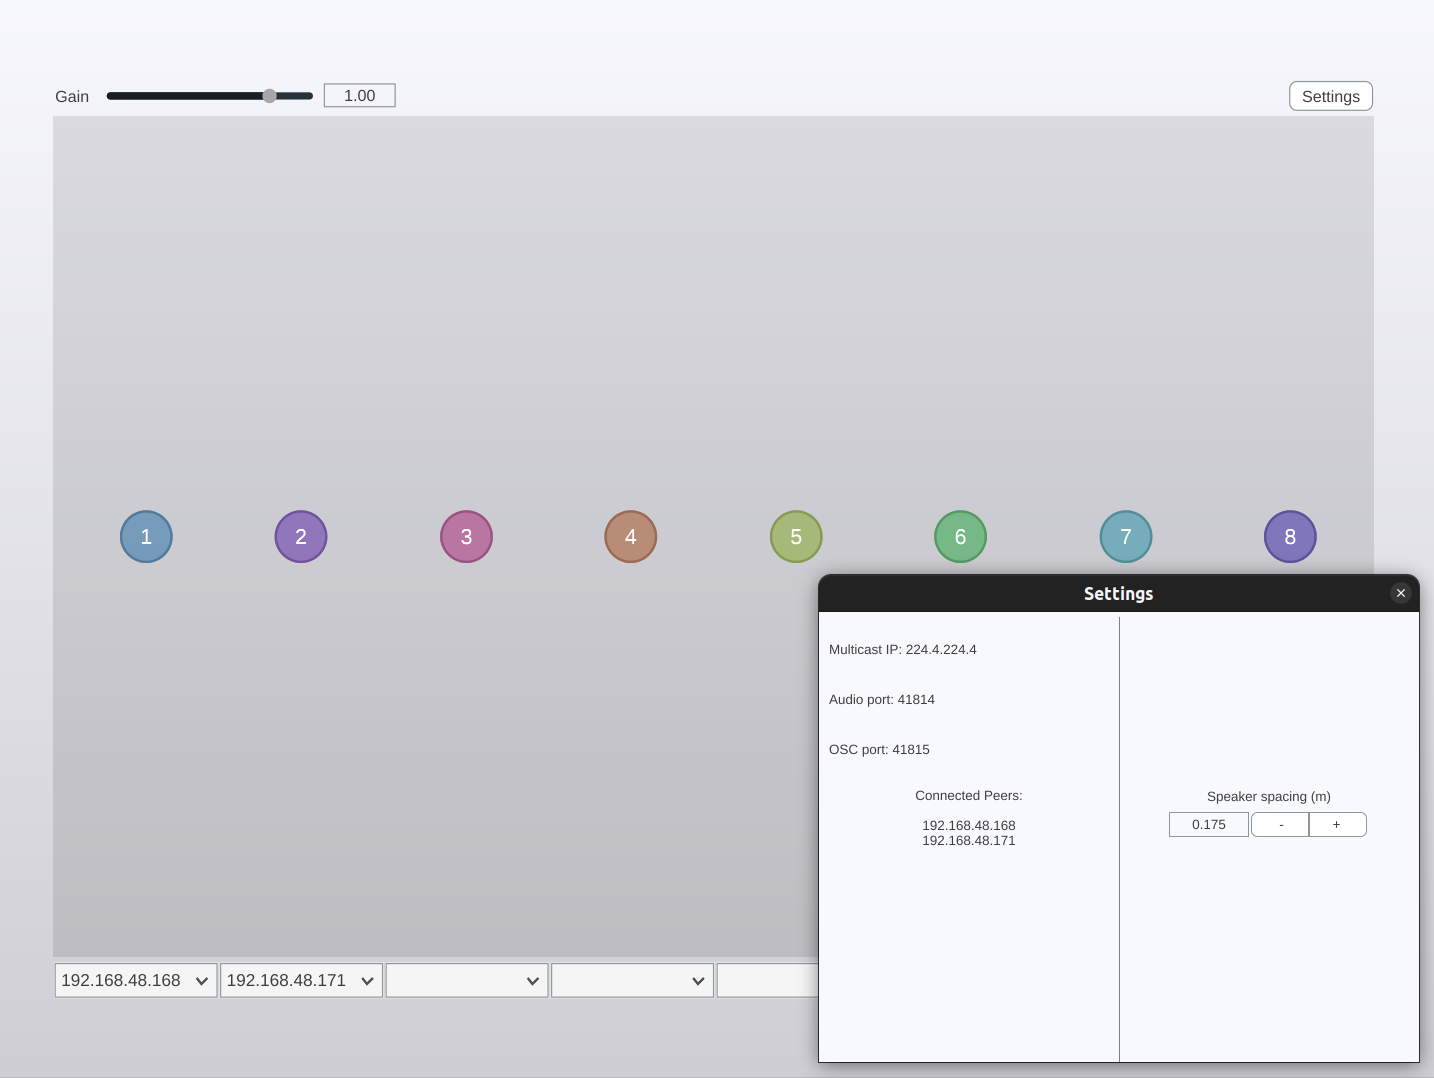
\includegraphics[width=\textwidth]{figures/plugin}
        \caption{
            User interface for the WFS controller DAW plugin, with modal
            settings window visible.
            The interface consists of an X/Y control surface, with eight nodes
            representing the coordinates, normalised to $x,y \in [0,1]$, of sound
            sources in a virtual sound field.
            Dropdown menus at the bottom of the interface correspond with hardware
            module positions in the loudspeaker array; there are eight such menus
            in total, each associated hardware module producing output for two
            loudspeakers.
            The settings window facilitates specifying the speaker spacing, and
            shows a list of connected network peers.
        }
        \label{fig:plugin-interface}
    \end{figure}

    Server-side, the software system consists of a VST plugin running in Reaper
    digital audio workstation software.\footnote{\url{https://reaper.fm/}}
    The plugin comprises the networked audio server, receiving monophonic audio
    sources in the form of audio or instrument tracks in the DAW, plus a control
    data server, commanded either by parameter automation via the DAW, or manually
    via a graphical user interface (see \figref{fig:plugin-interface}).
    The audio and control data servers send streams of UDP packets to a UDP
    multicast group.

    Client-side software connects to the multicast group and reads UDP packets
    containing audio and control data from the server.
    These streams are delivered to the Faust-based WFS algorithm, with audio
    streams processed according to the control parameters of virtual sound source
    positions and speaker spacing.
    The WFS algorithm produces driving signals for each of the two output channels
    of the hardware module on which it is running.
    Additionally, the client-side networked audio client returns a stream of audio
    data to the multicast group, to be consumed by the server.

    Code for the server and client software components can be found at
    \url{https://github.com/hatchjaw/netjuce} and
    \url{https://github.com/hatchjaw/netjuce-teensy} respectively.


    \section{Results}\label{sec:results}

    \begin{figure}[ht]
        \centering
        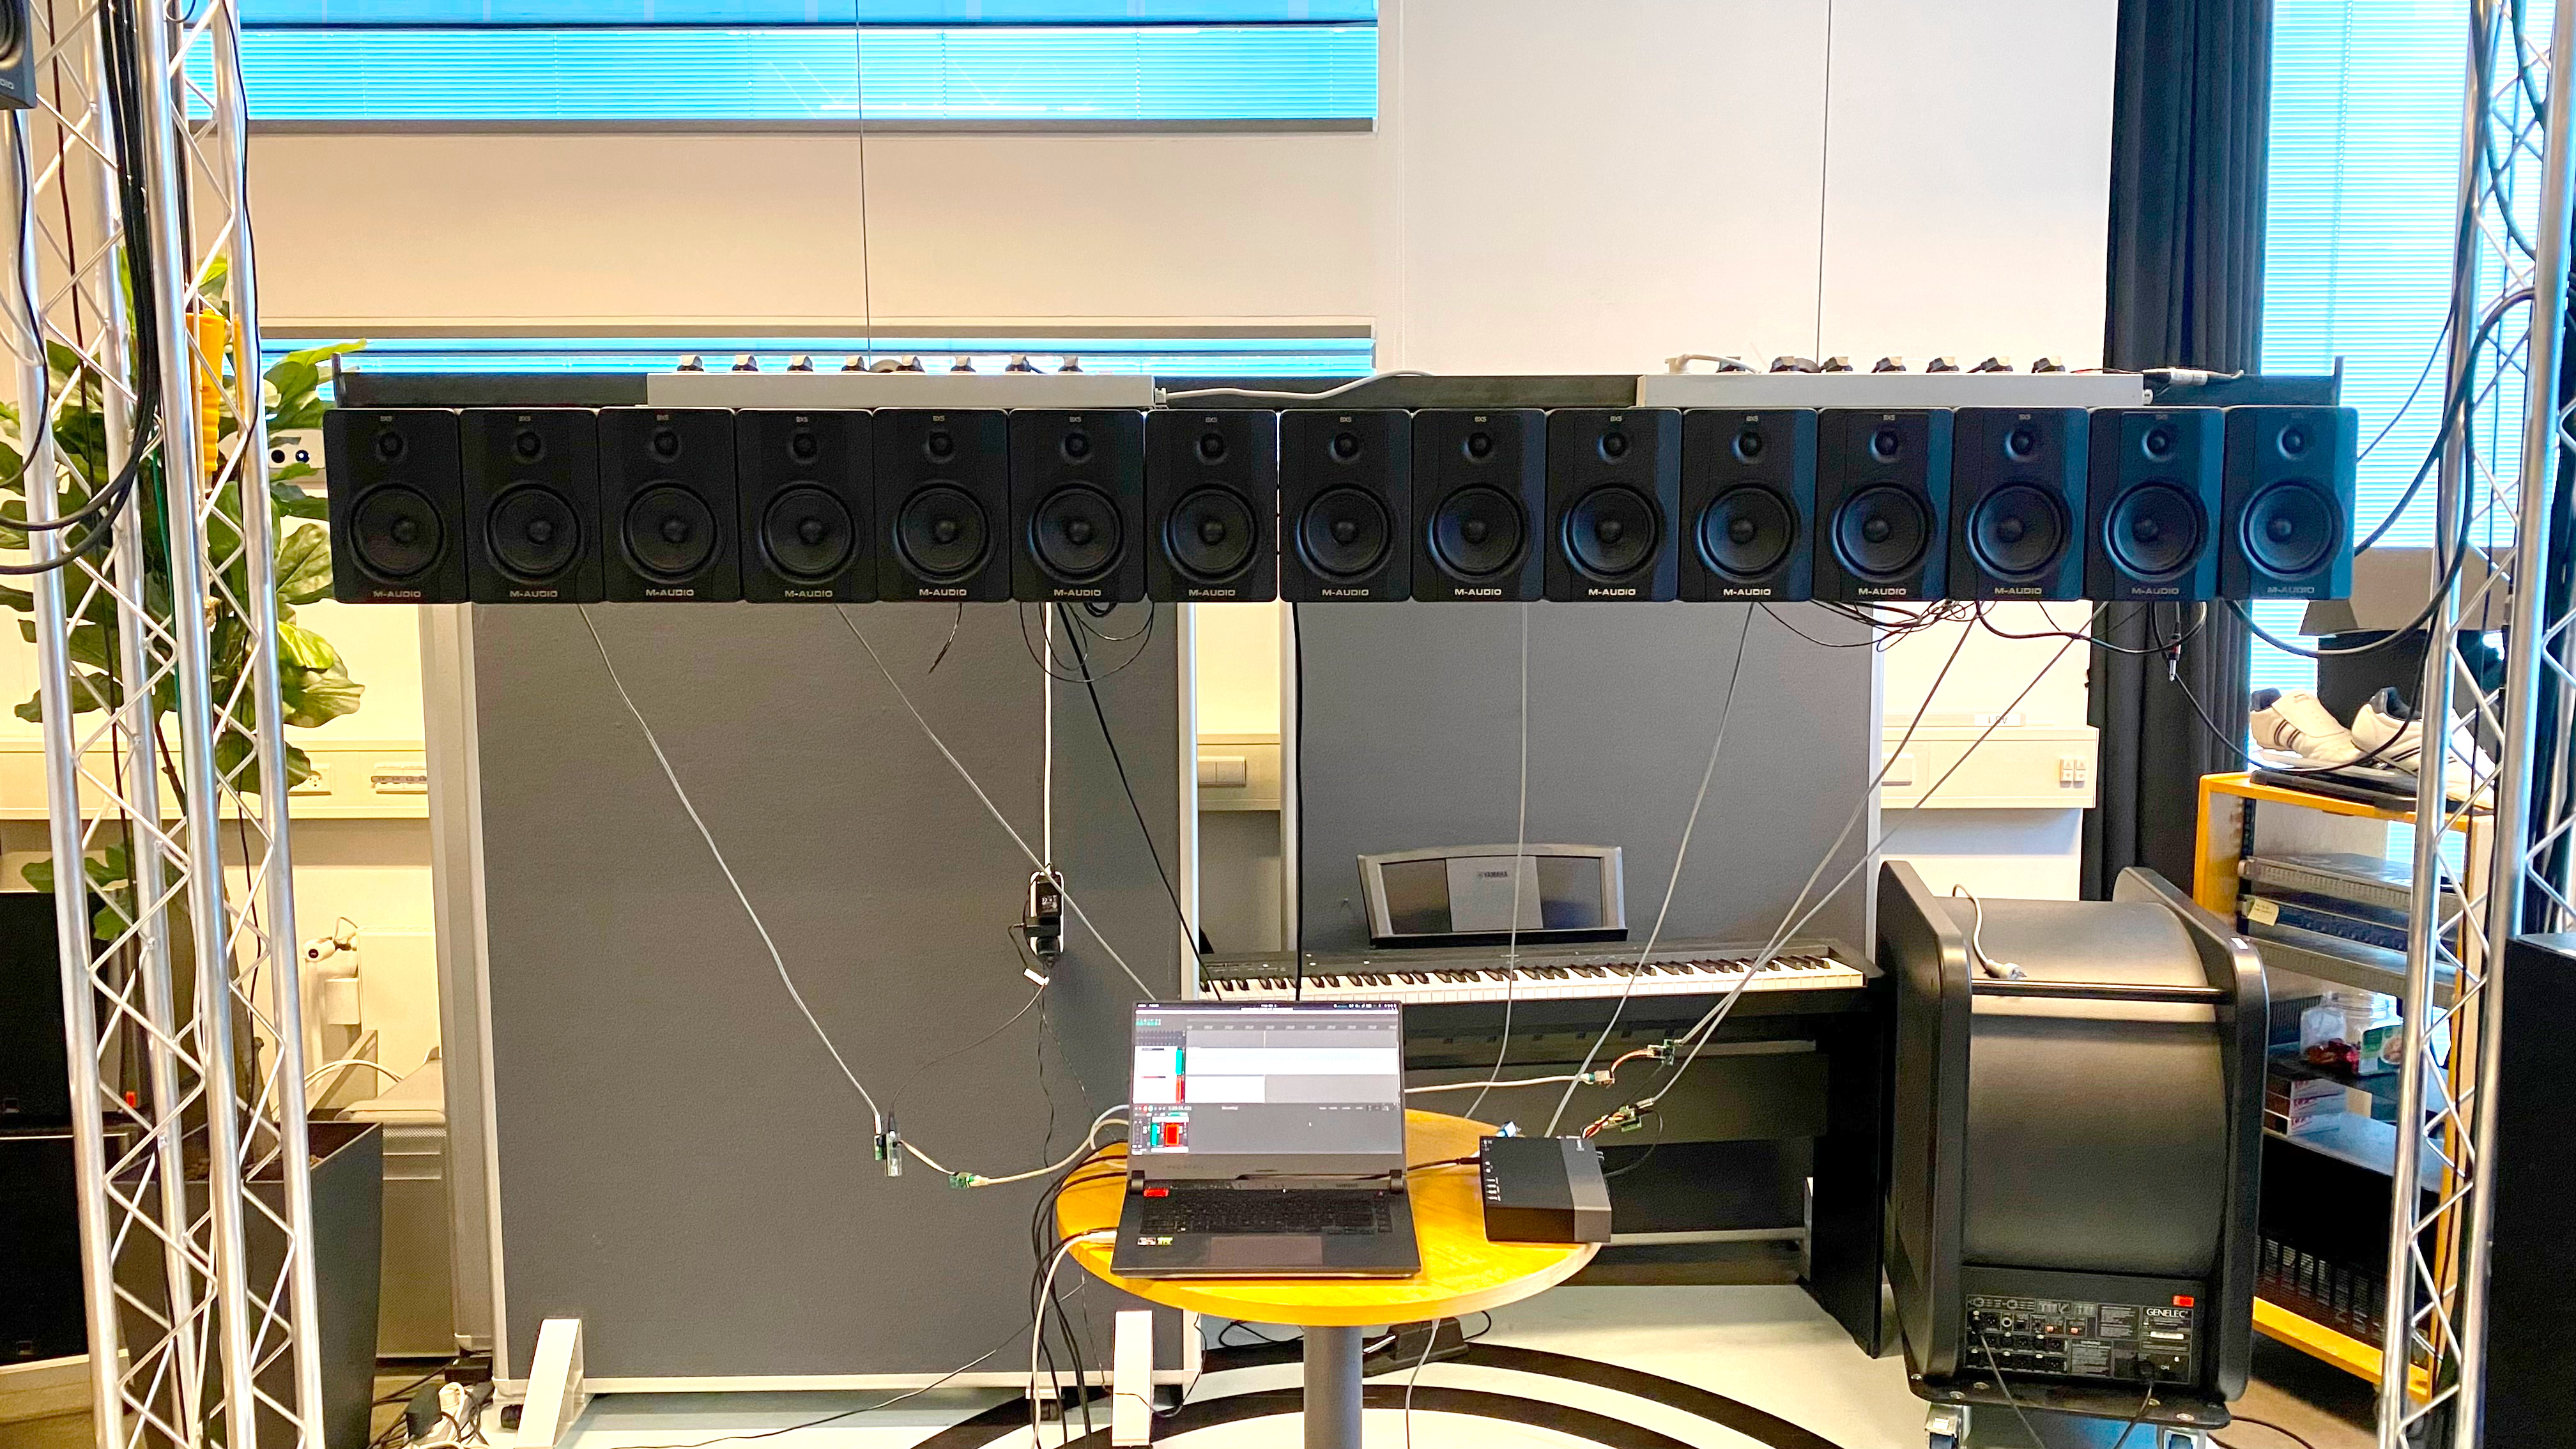
\includegraphics[width=\textwidth]{figures/eval-setup}
        \caption{
            System configuration for technical and perceptual evaluation.
            Eight hardware modules connected to fifteen loudspeakers \textemdash{}
            seven of the modules produced output for two loudspeakers each; the
            final module used only its first output channel.
        }
        \label{fig:eval-setup}
    \end{figure}

    Possessing technical underpinnings, but ultimately being designed to
    serve immersive auditory ends, it was important to consider the performance of
    the system described and developed in \secref{sec:method} in terms of
    both its technical capabilities and the quality of the perceptual effects it
    was able to support.
    The success of the system as a platform for audio spatialisation techniques is
    contingent on it being composed of effective solutions to the challenges posed
    by distributing audio processing across a local area network.
    It is of limited worth, however, as a technical exercise in isolation;
    the subjective assessment of listeners may help identify the most critical
    aspects of the technical implementation and guide future development.

    \subsection{Technical Evaluation}\label{subsec:technical-evaluation}

    \begin{figure}[ht]
        \centering
        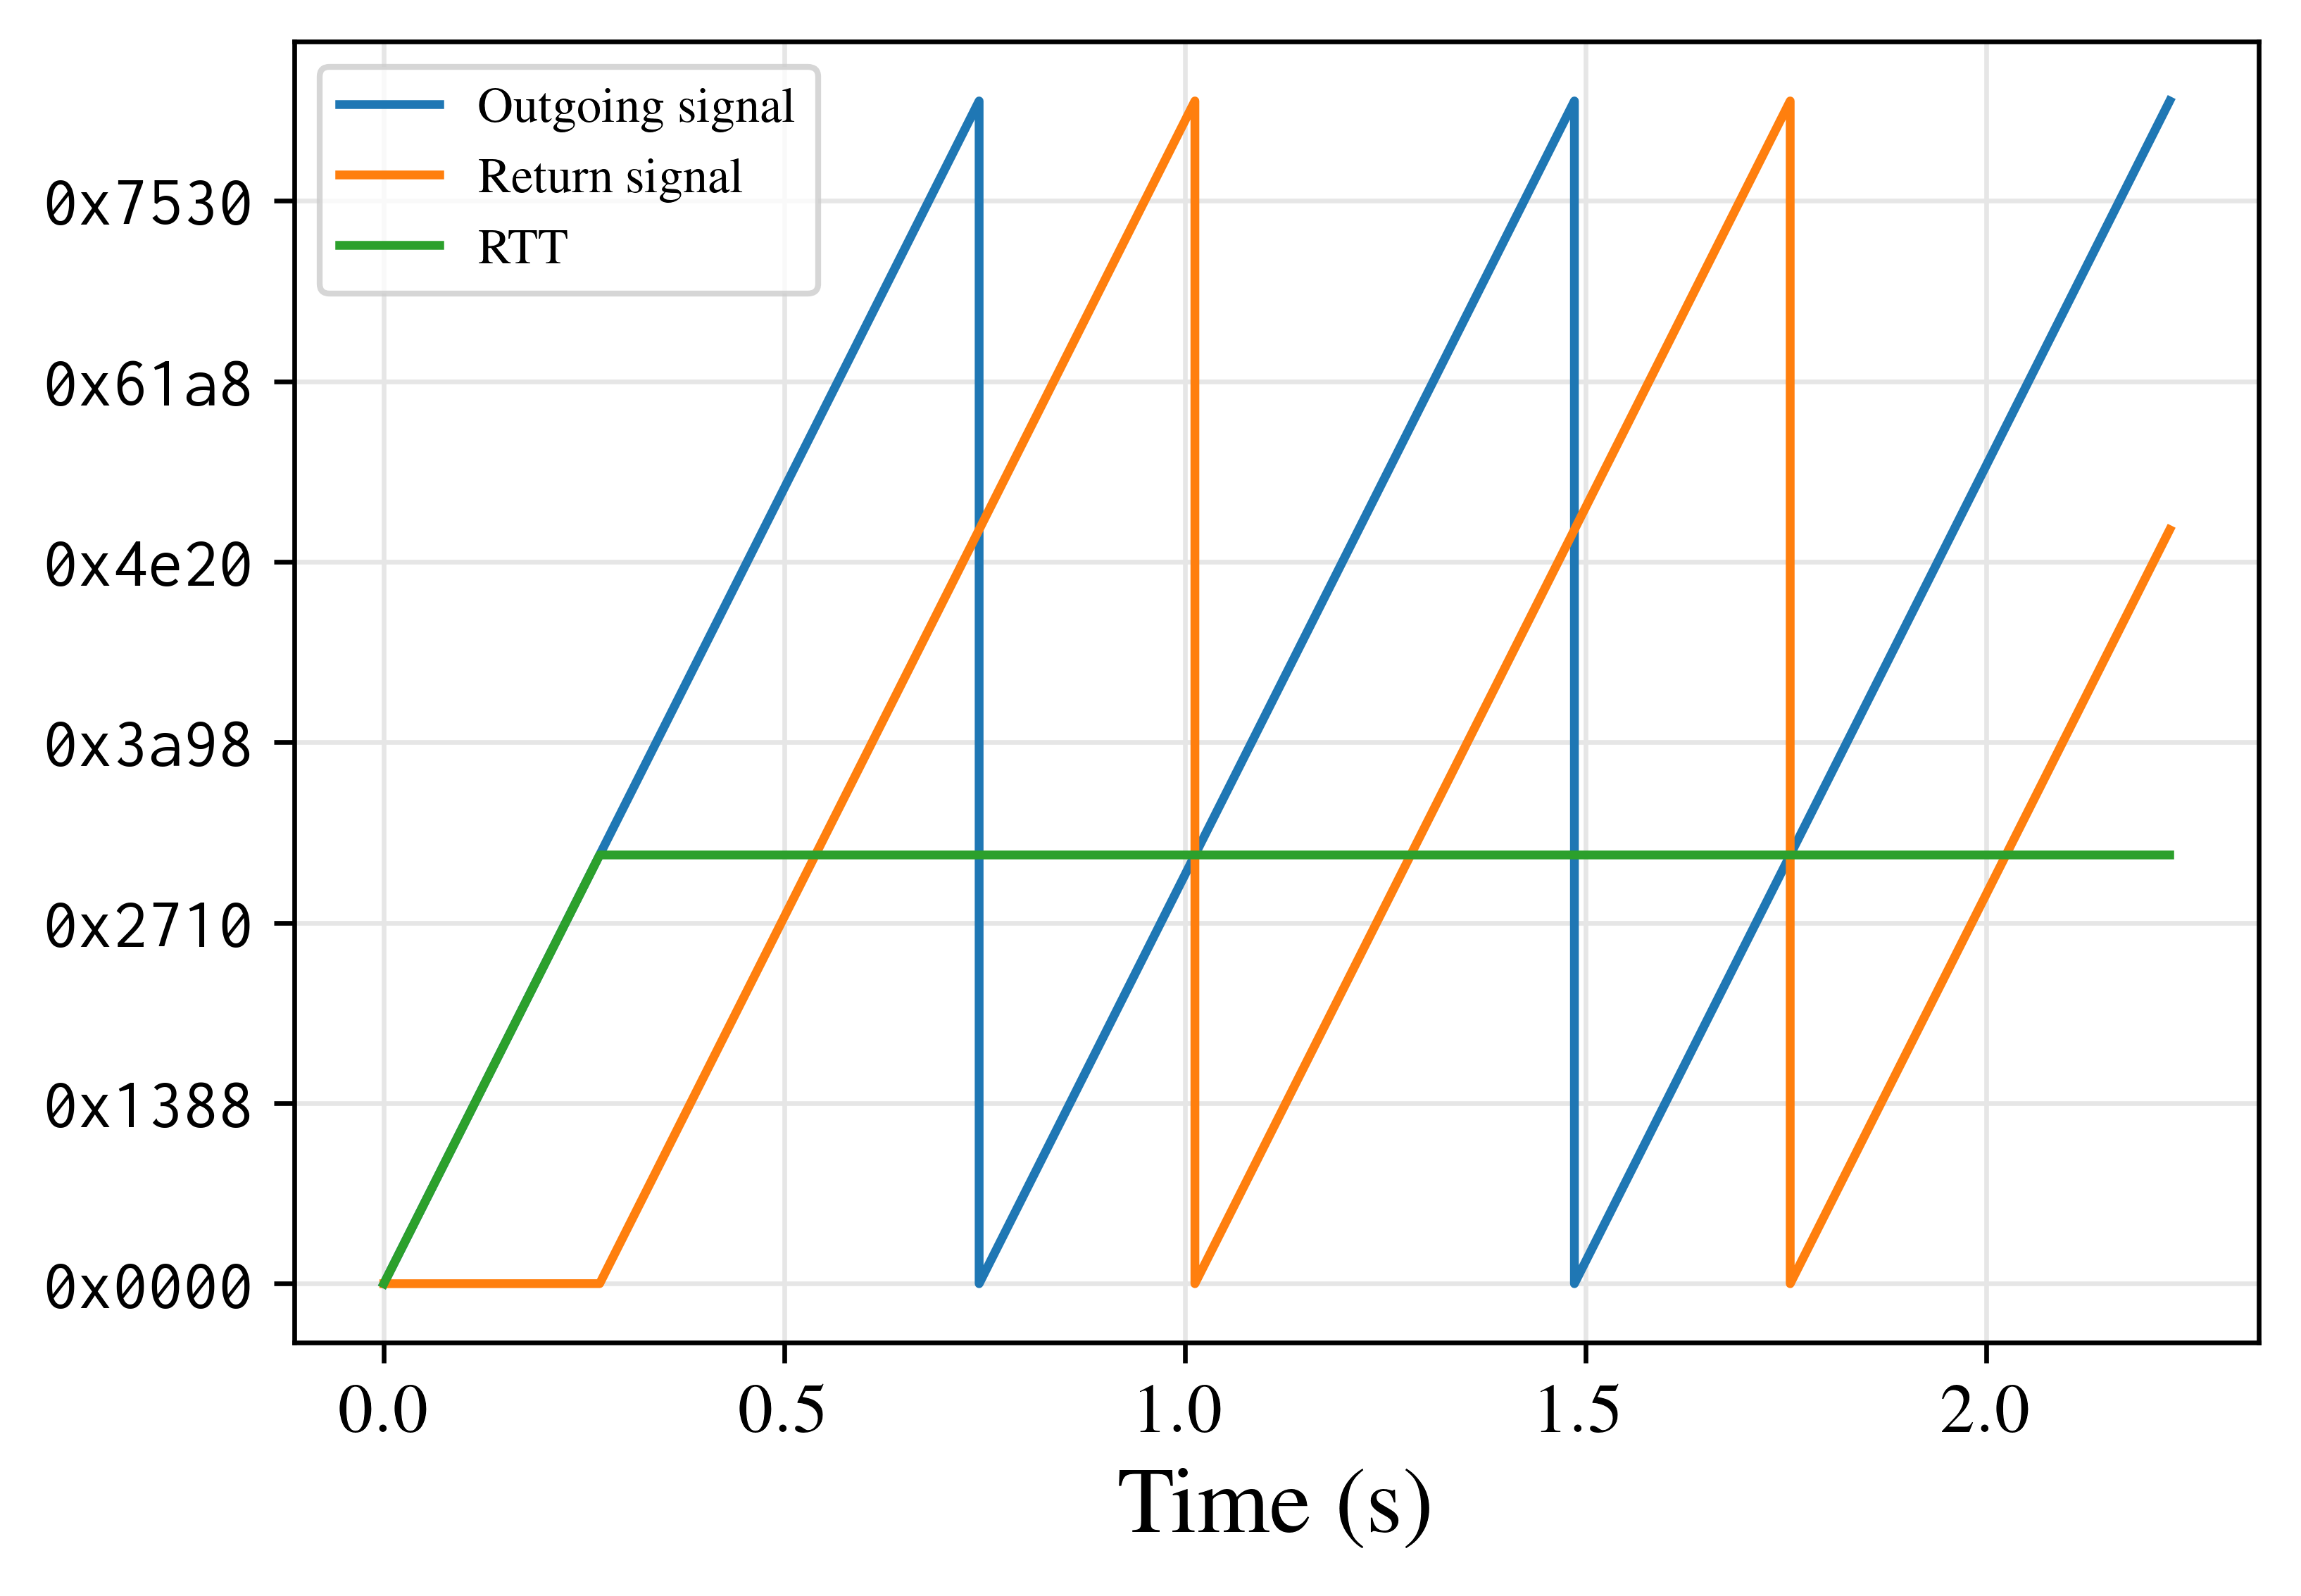
\includegraphics[width=.5\textwidth]{figures/test-signal}
        \caption{
            Illustration of the use of a test signal, a unipolar sawtooth wave,
            to measure round trip time.
            Subtracting the return signal from the outgoing signal gives the time
            (in samples) between transmission and reception.
        }
        \label{fig:test-signal}
    \end{figure}
    \noindent
    Of most pressing technical concern is the matter of synchronicity between the
    hardware modules.
    To assess this, a similar approach was taken to that found
    in~\citep{rushton_microcontroller-based_2023}
    and~\citep{gabrielli_networked_2012}.

    \subsubsection{Round Trip Time}
    To measure transmission round trip time (RTT), the server transmitted a unipolar
    sawtooth wave of unit amplitude increment to the multicast group, and each
    client, upon receiving the signal simply returned it immediately to the group to
    be read by the server.
    At the server side, the return signal, $x_{\text{ret}}$, was subtracted from the
    outgoing signal, $x_{\text{out}}$, at the time of reception, with round trip
    time found as:
    \begin{equation}
        \label{eq:rtt}
        \text{RTT} = \begin{cases}
                         x_{\text{out}} + \max_{\text{int16}} - x_{\text{ret}}, &x_{\text{out}} < x_{\text{ret}}, \\
                         x_{\text{out}} - x_{\text{ret}}, &\text{otherwise},
        \end{cases}
    \end{equation}
    where $\max_{\text{int16}}$ is the maximum value representable by a
    signed 16-bit integer, \texttt{0x7fff} (\numDec{32767}).

    The resulting value is the number of samples elapsed between transmission and
    reception (see \figref{fig:test-signal}).
    Since there is one source of transmission, for multiple clients, comparing RTT
    offers a means to assess inter-client synchronicity.
    Server-to-client latency cannot be measured in this way, but that can be
    inferred to be around half of, and, of course, certainly not greater than, the
    RTT.\

    \begin{figure}[h]
        \centering
        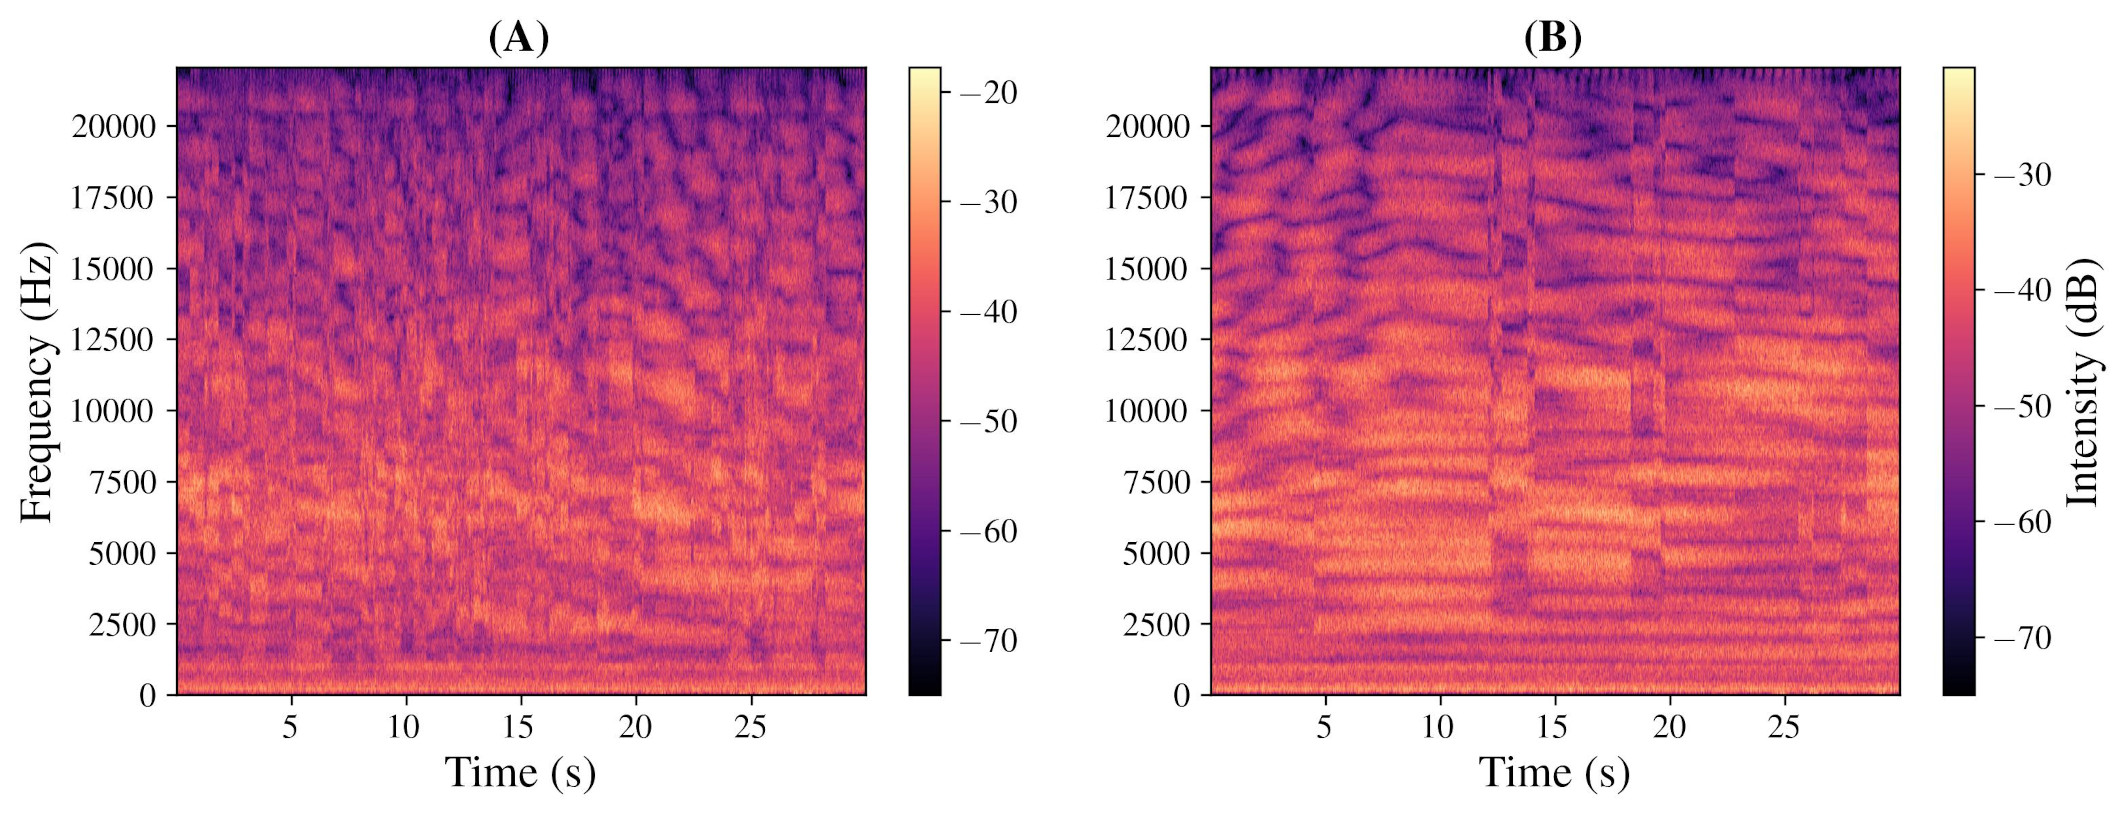
\includegraphics[width=\textwidth]{figures/wgn_specgram_16_32}
        \caption{
            Magnitude spectrograms of ambient, monophonic recordings of a
            reproduction of white Gaussian noise by a group of eight networked
            audio clients driving an array of fifteen loudspeakers spaced at
            intervals of \qty{.175}{\m}.
            Capacitor microphone placed $\sim$\qty{2}{\m} from the
            speaker array.
            Audio buffer size (A) 16 frames; (B) 32 frames.
        }
        \label{fig:spectrograms}
    \end{figure}

    \subsubsection{Clock Drift/Skew}
    A unipolar sawtooth wave of unit amplitude increment was generated on the
    clients, subtracted from the incoming sawtooth wave from the server, and the
    difference (found as per equation~\eqref{eq:rtt}) returned to the multicast
    group for consumption by the server.
    The incoming signal and the one being generated on a given client should, under
    ideal conditions, be out of phase by some constant value;
    if this value changes then relative drift has occurred between server and
    client.
    The client-side clock-adjustment strategy was designed to minimise the reliance
    on the adaptive resampling approach that it complements;
    low drift would be indicative of the effectiveness of that strategy.

    \begin{figure}[h]
        \centering
        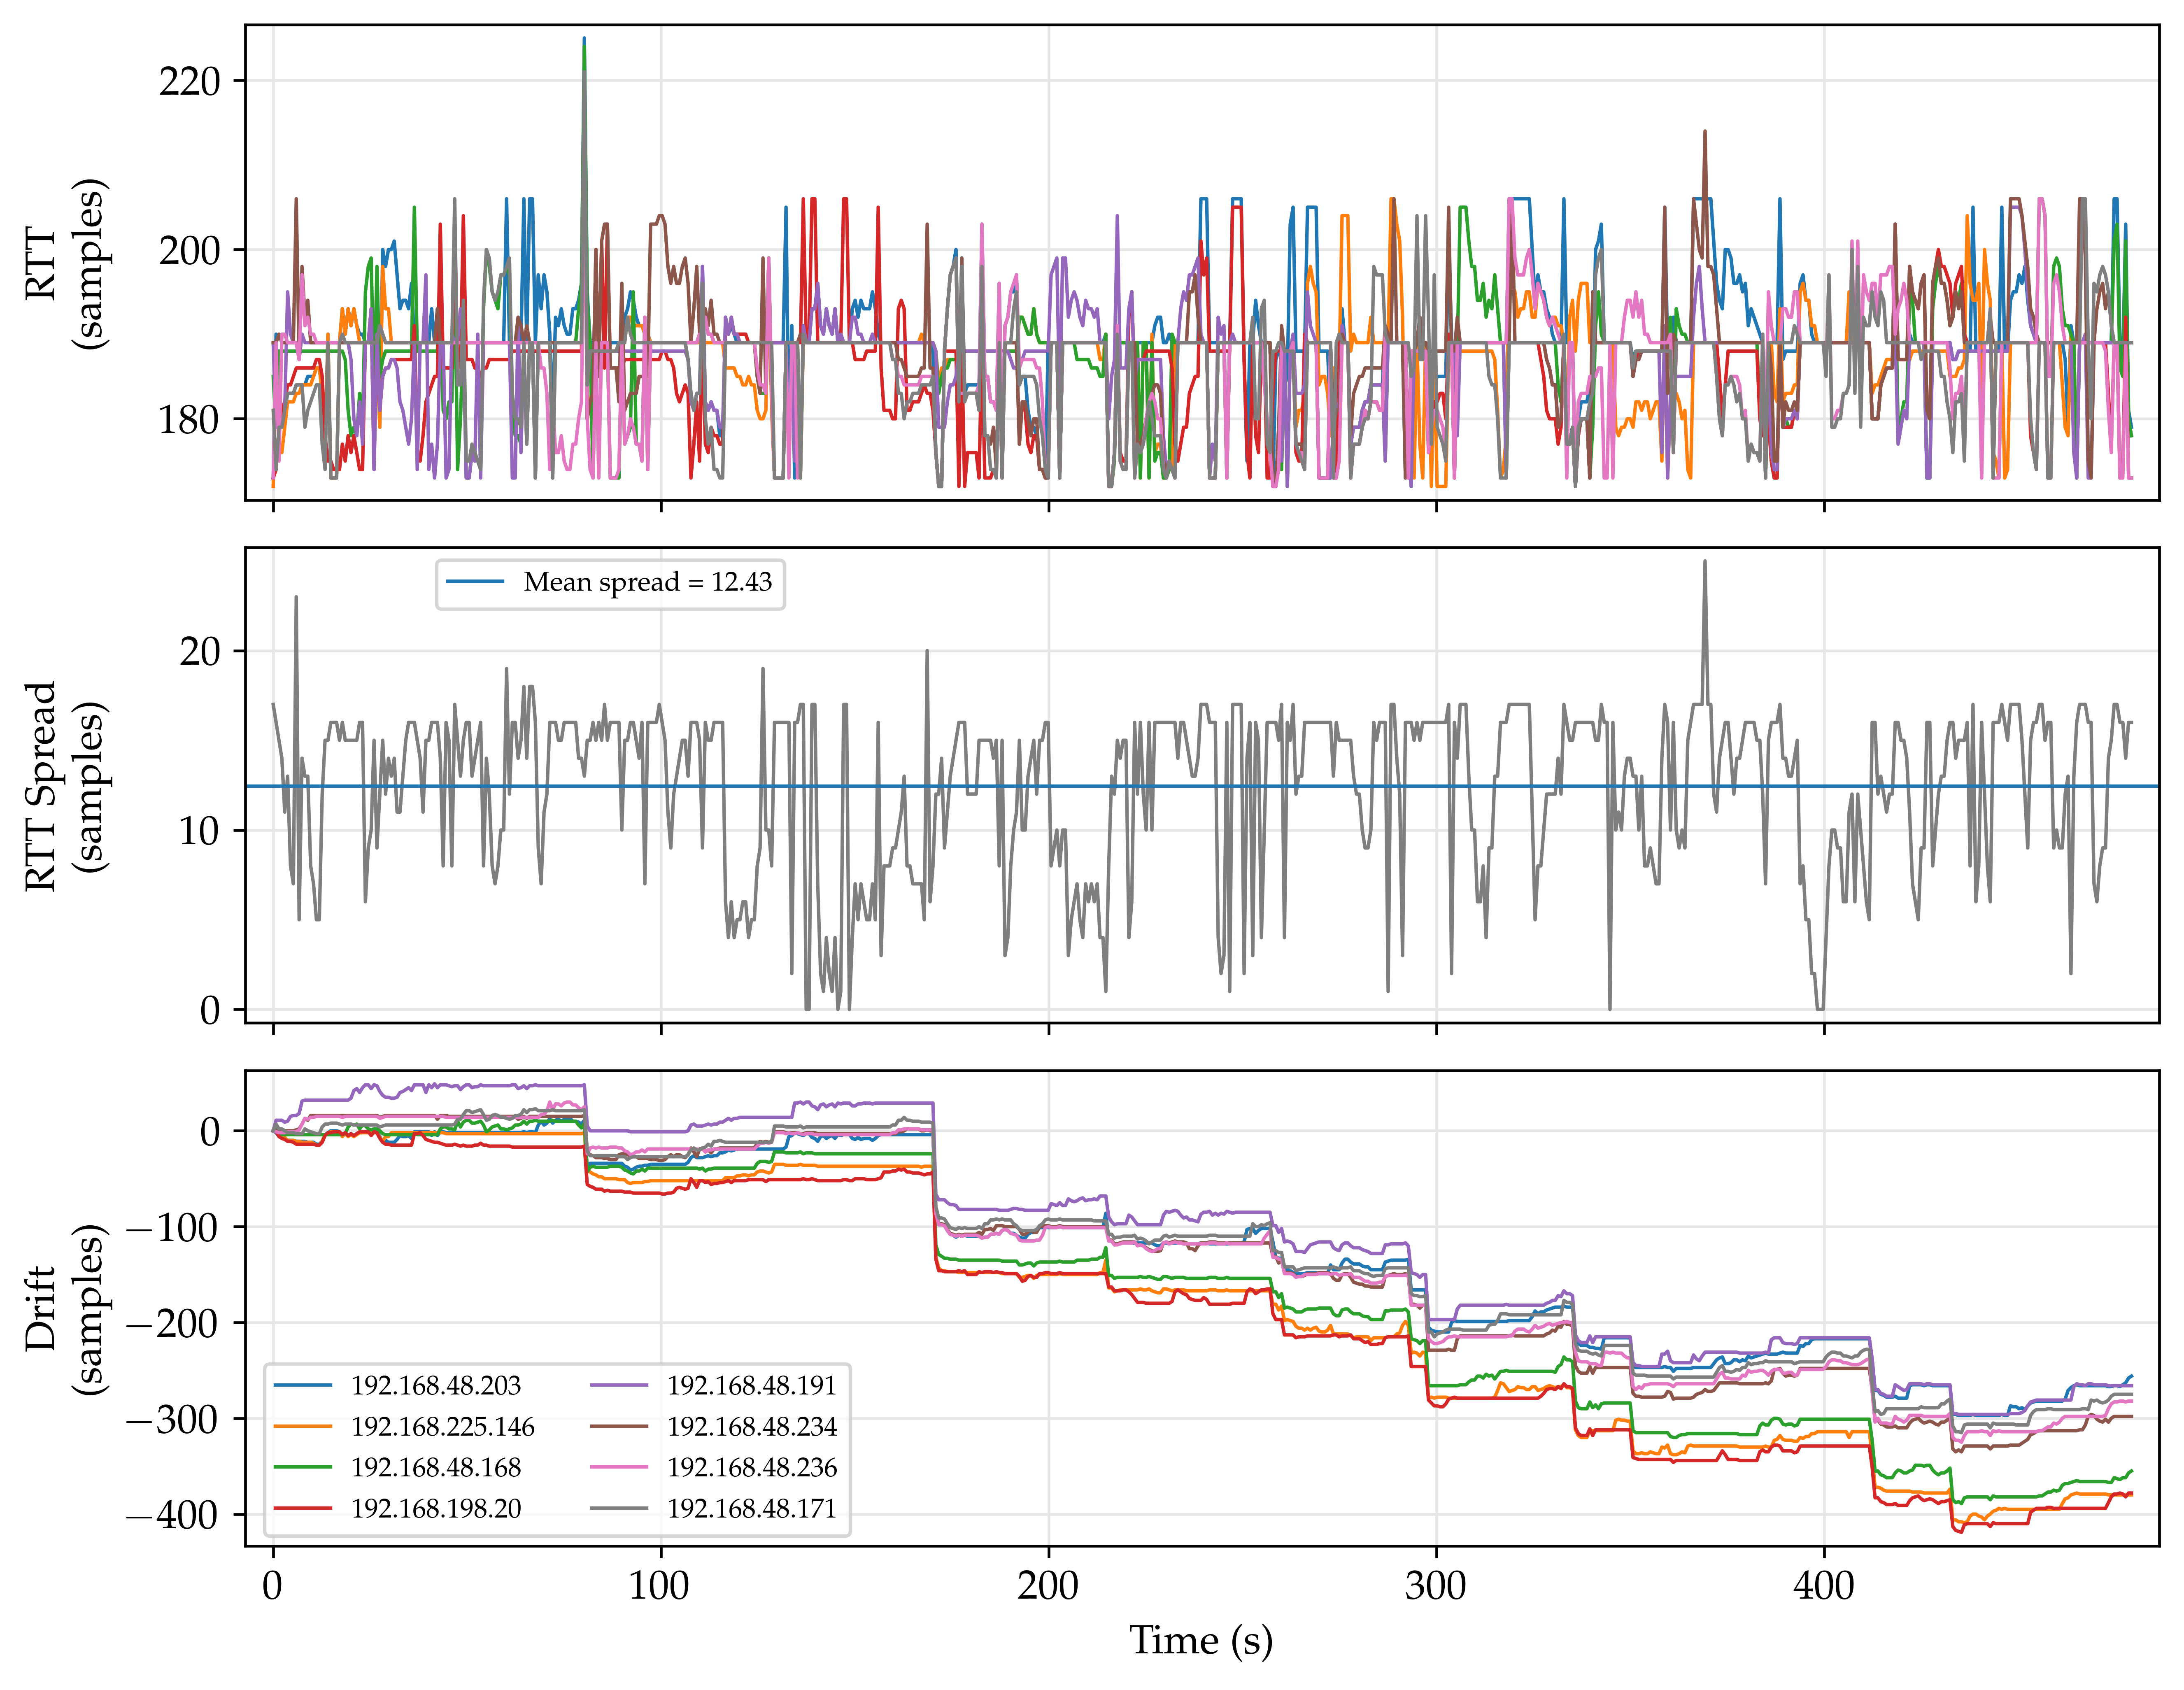
\includegraphics[width=\textwidth]{figures/rtt_drift_16}
        \caption{
            Round-trip time, RTT spread, and clock drift measurements for eight
            networked audio clients, for a networked audio session of eight minutes'
            duration.
            Audio buffer size, 16 frames, sampling rate \qty{44.1}{\kHz}.
            The legend in the bottommost plot applies also to the upper plot.
            Round-trip time, in samples, measured at the server, and found as the
            difference between an outgoing sawtooth wave and its returning
            counterparts from each of eight connected clients.
            Round-trip time spread found as the range ($\text{RTT}_{\max} -
            \text{RTT}_{\min}$), in samples, at each point in time, of
            round-trip times reported for all eight clients.
            Mean spread is the arithmetic mean of RTT spread values taken across
            the entire test.
            Drift, in samples, found as the difference between an outgoing sawtooth
            wave and a sawtooth wave generated on each client, that difference
            returned to the multicast group for consumption by the server.
        }
        \label{fig:rtt-drift-16}
    \end{figure}

    Initial RTT and relative drift measurements for eight clients are shown in
    \figref{fig:rtt-drift-16}.
    Mean RTT spread, describing the average temporal interval over which clients
    were distributed over the course of the test, is promising, the 12.43 sample
    interval corresponding with approximately \qty{282}{\us}.
    RTT is clustered around a respectable 190 samples ($\sim$\qty{4.3}{\ms}).

    That visual clustering, coupled with the apparent tendency for RTT spread to
    lie at around 16 samples (i.e.\ precisely one buffer), suggest, however, a
    certain over-aggressiveness in the resampling strategy, perhaps resulting in a
    polarisation of clients to the temporal extremes of the interval between their
    audio interrupts.
    What \figref{fig:rtt-drift-16} does not show, and, given the short timescales
    involved, is not easily represented in such a diagram, is the rate of relative
    inter-client movement, i.e.\ the rate of change of asynchronicity.
    Subjective assessment of the system's audible output revealed that, given the
    rapid rate of relative movement between clients, in this state it would not
    stand up to perceptual testing.

    Transmitting a white Gaussian noise signal to the clients and delivering this to
    their audio outputs without further processing \textemdash{} seeking,
    essentially, to sonify QoS \textemdash{} an aggressive phasing, or time-varying
    comb-filter effect was clearly audible.
    This effect is visualised in \figref{fig:spectrograms}(A);
    ideally (subject to the frequency response of the microphone used) an ambient
    recording of a white noise source would correspond with a magnitude spectrogram
    exhibiting equal intensity across the frequency range at all times;
    clearly, though, there are regions of greater and lesser intensity, and these
    regions shift and change rapidly over time.
    In addition to the above, tests involving the reproduction of signals
    containing steady-state harmonic content revealed obtrusive audible artefacts.

    \begin{figure}[h]
        \centering
        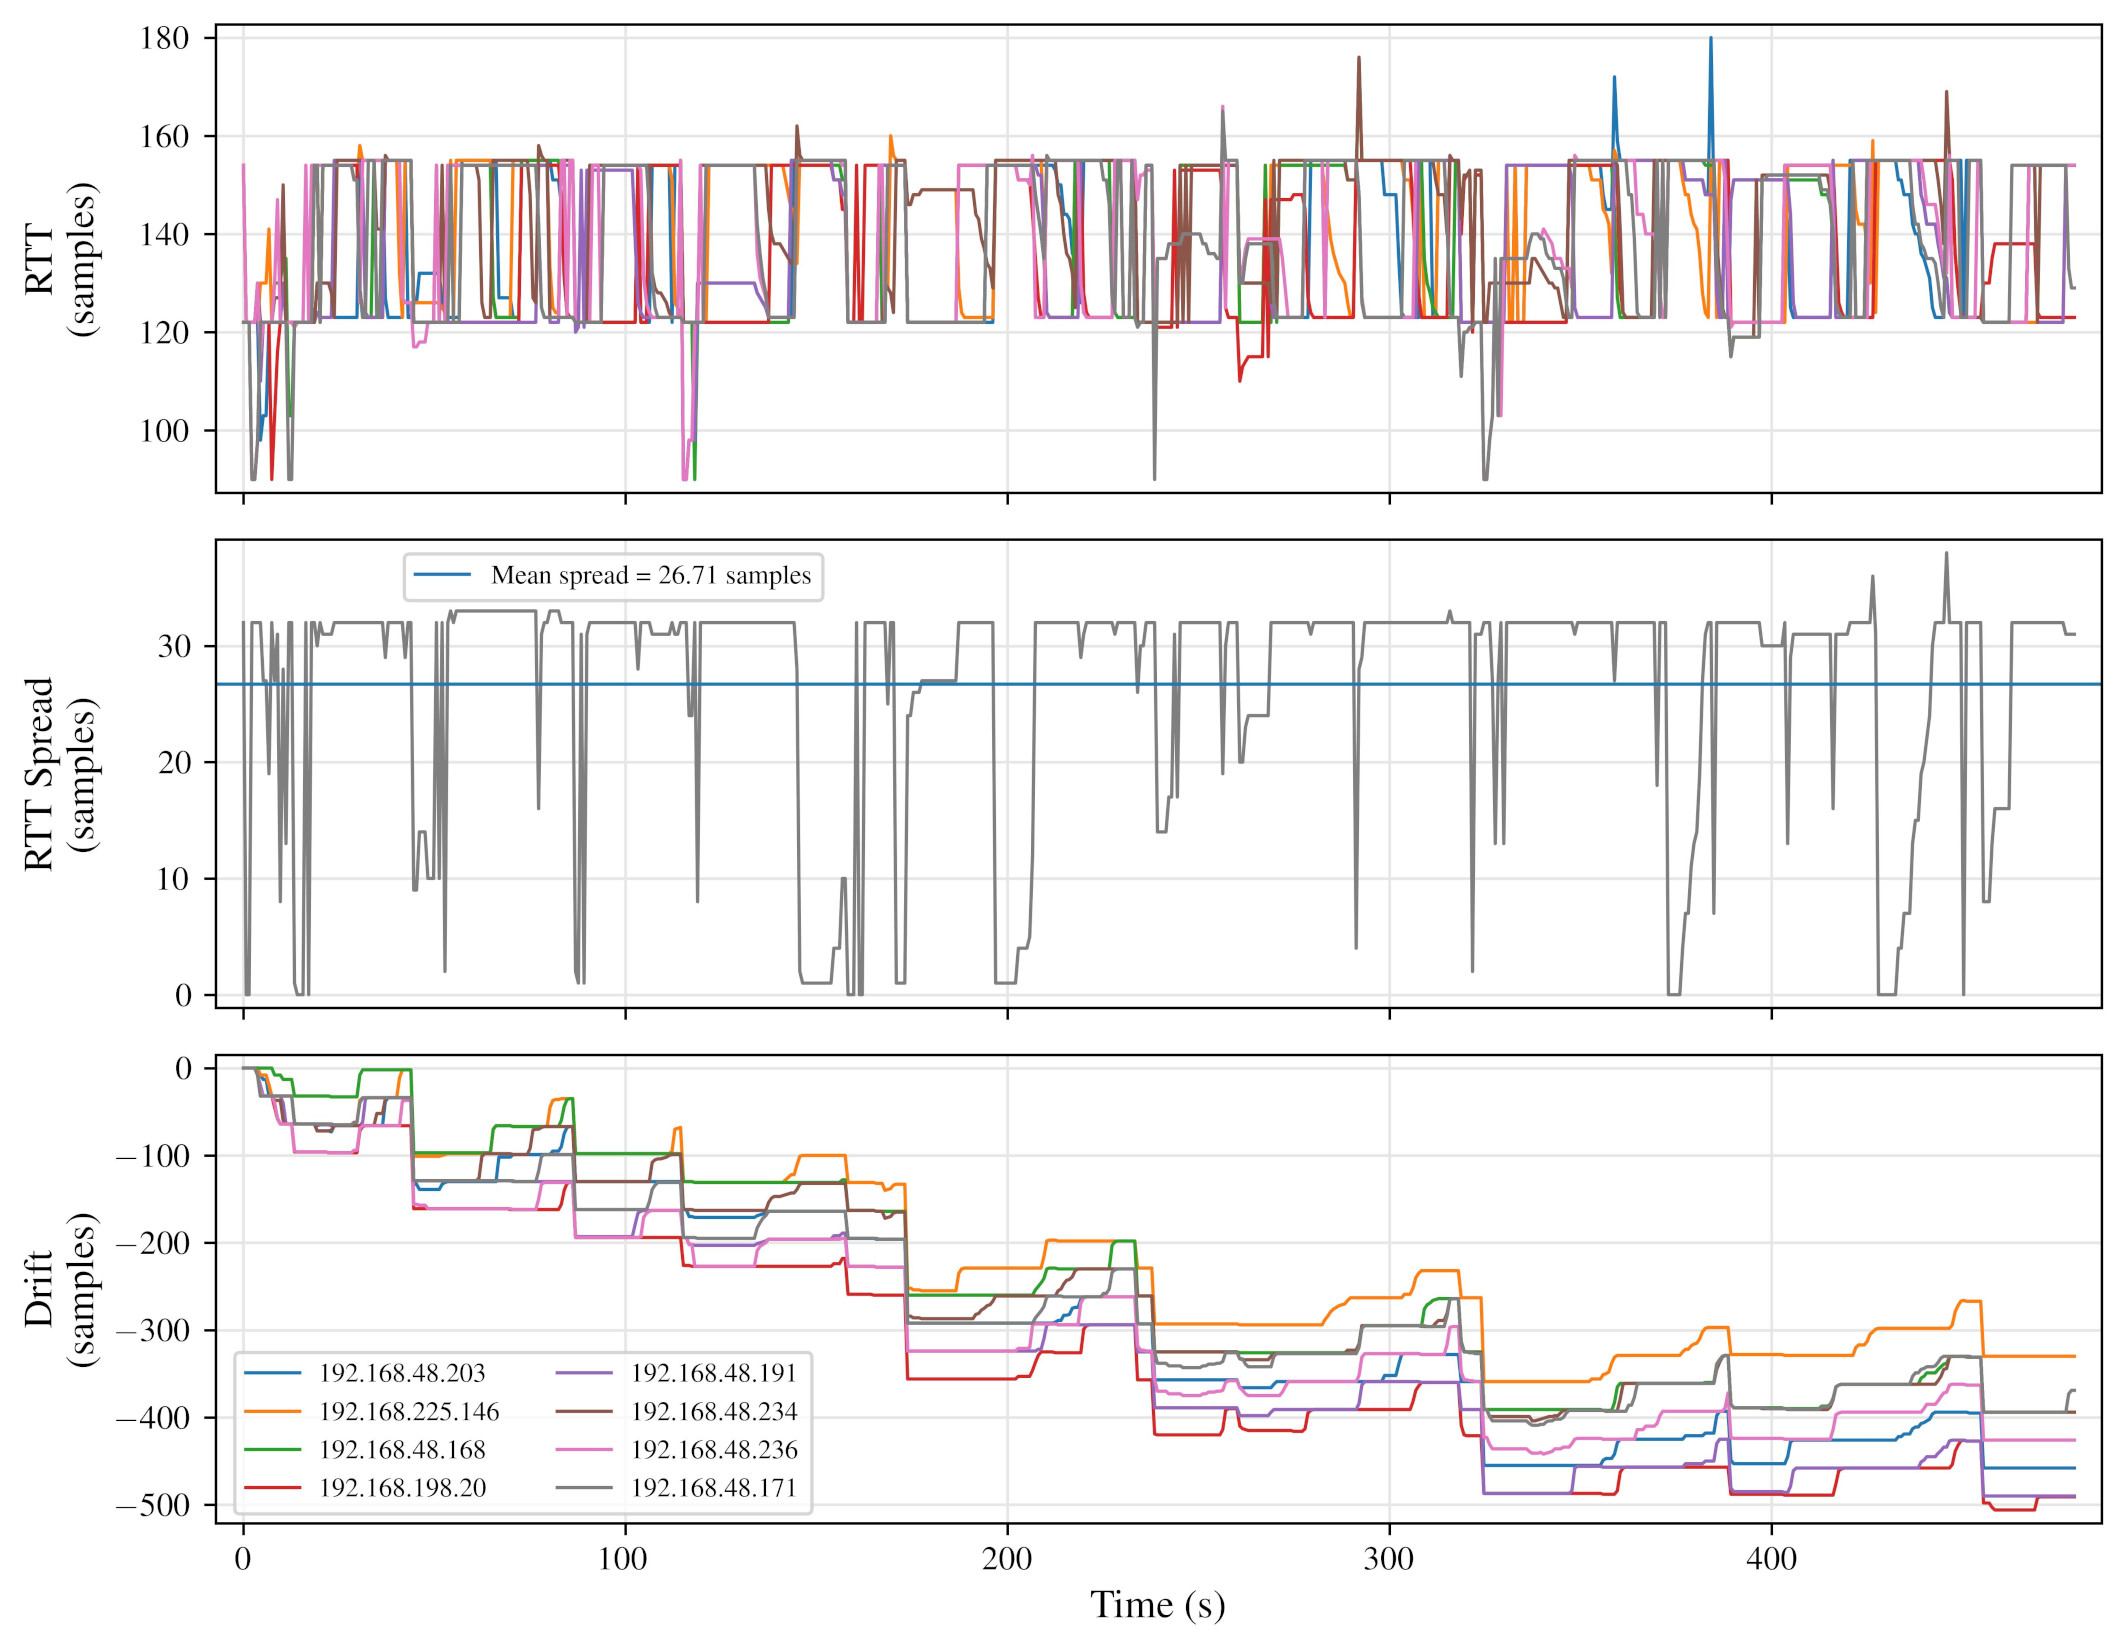
\includegraphics[width=\textwidth]{figures/rtt_drift_32}
        \caption{
            Round-trip time, RTT spread, and clock drift measurements
            for eight networked audio clients, for a networked audio session of
            eight minutes' duration.
            Audio buffer size, 32 frames.
        }
        \label{fig:rtt-drift-32}
    \end{figure}

    A buffer size of 16 frames had been selected in an attempt to minimise the
    duration of the window of inter-client synchronicity, and to maximise the
    number of channels that could be transmitted over the network, subject to
    restrictions posed by the MTU (see
    \secref{subsubsec:transmission-considerations}).
    Recalling, however, that previous
    work~\citep{rushton_microcontroller-based_2023}
    had employed a 32-frame audio buffer, equivalent measurements were taken for
    the larger buffer size, the results of which are depicted in
    \figref{fig:rtt-drift-32} and \figref{fig:spectrograms}(B).

    Again, visually, there is an apparent clustering in the RTT recordings, with
    clients spending large periods separated by around one buffer's worth of
    samples ($\sim$\qty{726}{\us}), seemingly often grouped at either
    extreme of the interval of one audio buffer.
    The mean RTT spread, equating to $\sim$\qty{626}{\us}, is comparable with
    results from prior work.
    Importantly, however, and as demonstrated in \figref{fig:spectrograms}(B), the
    rate of relative inter-client temporal movement was much improved by the switch
    to a 32-frame buffer.
    Although exhibiting similar visual striations to the spectrogram for the test
    at 16 frames, fluctuations occur less frequently, and seemingly more
    gradually.
    Indeed, subjectively-speaking, the disruption caused by the phasing effect
    that afflicted the 16-frame buffer implementation was significantly reduced,
    as was the presence of audible artefacts affecting harmonic signals.
    Thus it was the version of the system employing a buffer size of 32 frames
    that was exposed to perceptual evaluation.

    Clock drift measurements in \figsref{fig:rtt-drift-16}{fig:rtt-drift-32} exhibit
    comparable trends.
    Increasing negative drift over time is indicative of the clients running faster
    than the server.
    Visually, there is evidence that client clocks adjust to approximate parity
    with the server for periods of time, perhaps falling slightly slower (e.g.\
    the drift plot in \figref{fig:rtt-drift-16}, between 90 and 160 seconds), but
    intermittently demonstrate leaps, the largest of which are in the negative
    direction.

    \subsubsection{Discussion}\label{subsubsec:discussion-tech}

    The temporal clustering and polarisation seen in
    \figsref{fig:rtt-drift-16}{fig:rtt-drift-32} is indicative of two points for
    improvement with regard to technical implementation:
    the read-write difference threshold strategy may be insufficiently forgiving,
    forcing the read position into rapid changes in response to periods of jitter;
    and without an authoritative clock to indicate to the clients when each block of
    audio data should be output, even if clock rates were perfectly aligned, there
    is nothing to guarantee agreement of the timing of audio interrupts at the
    client side.

    The steps seen in the drift plots in
    \figsref{fig:rtt-drift-16}{fig:rtt-drift-32} appear (particularly in
    \figref{fig:rtt-drift-32}) to occur in multiples of the audio buffer size.
    This suggests either packet loss or, more likely,\footnote{
        During many hours of testing, no instance of packet loss was reported by any
        of the clients.
    } moments of pronounced jitter, causing
    clients to rapidly reduce (or, less commonly, increase) their read-position
    increment to maintain the read-write delta.
    One may expect such a phenomenon to be followed by an immediate rebound, but
    this appears to be a more gradual process.
    The overall trend, for this combination of server and clients at least, is for
    clients to run faster than the server;
    the clock adjustment strategy employed relies on inferring time from the rate of
    packet transmission, which may not offer sufficient temporal resolution for
    accurate drift compensation.

    \subsection{Perceptual Evaluation}\label{subsec:perceptual-evaluation}

    \begin{figure}[h!]
        \centering
        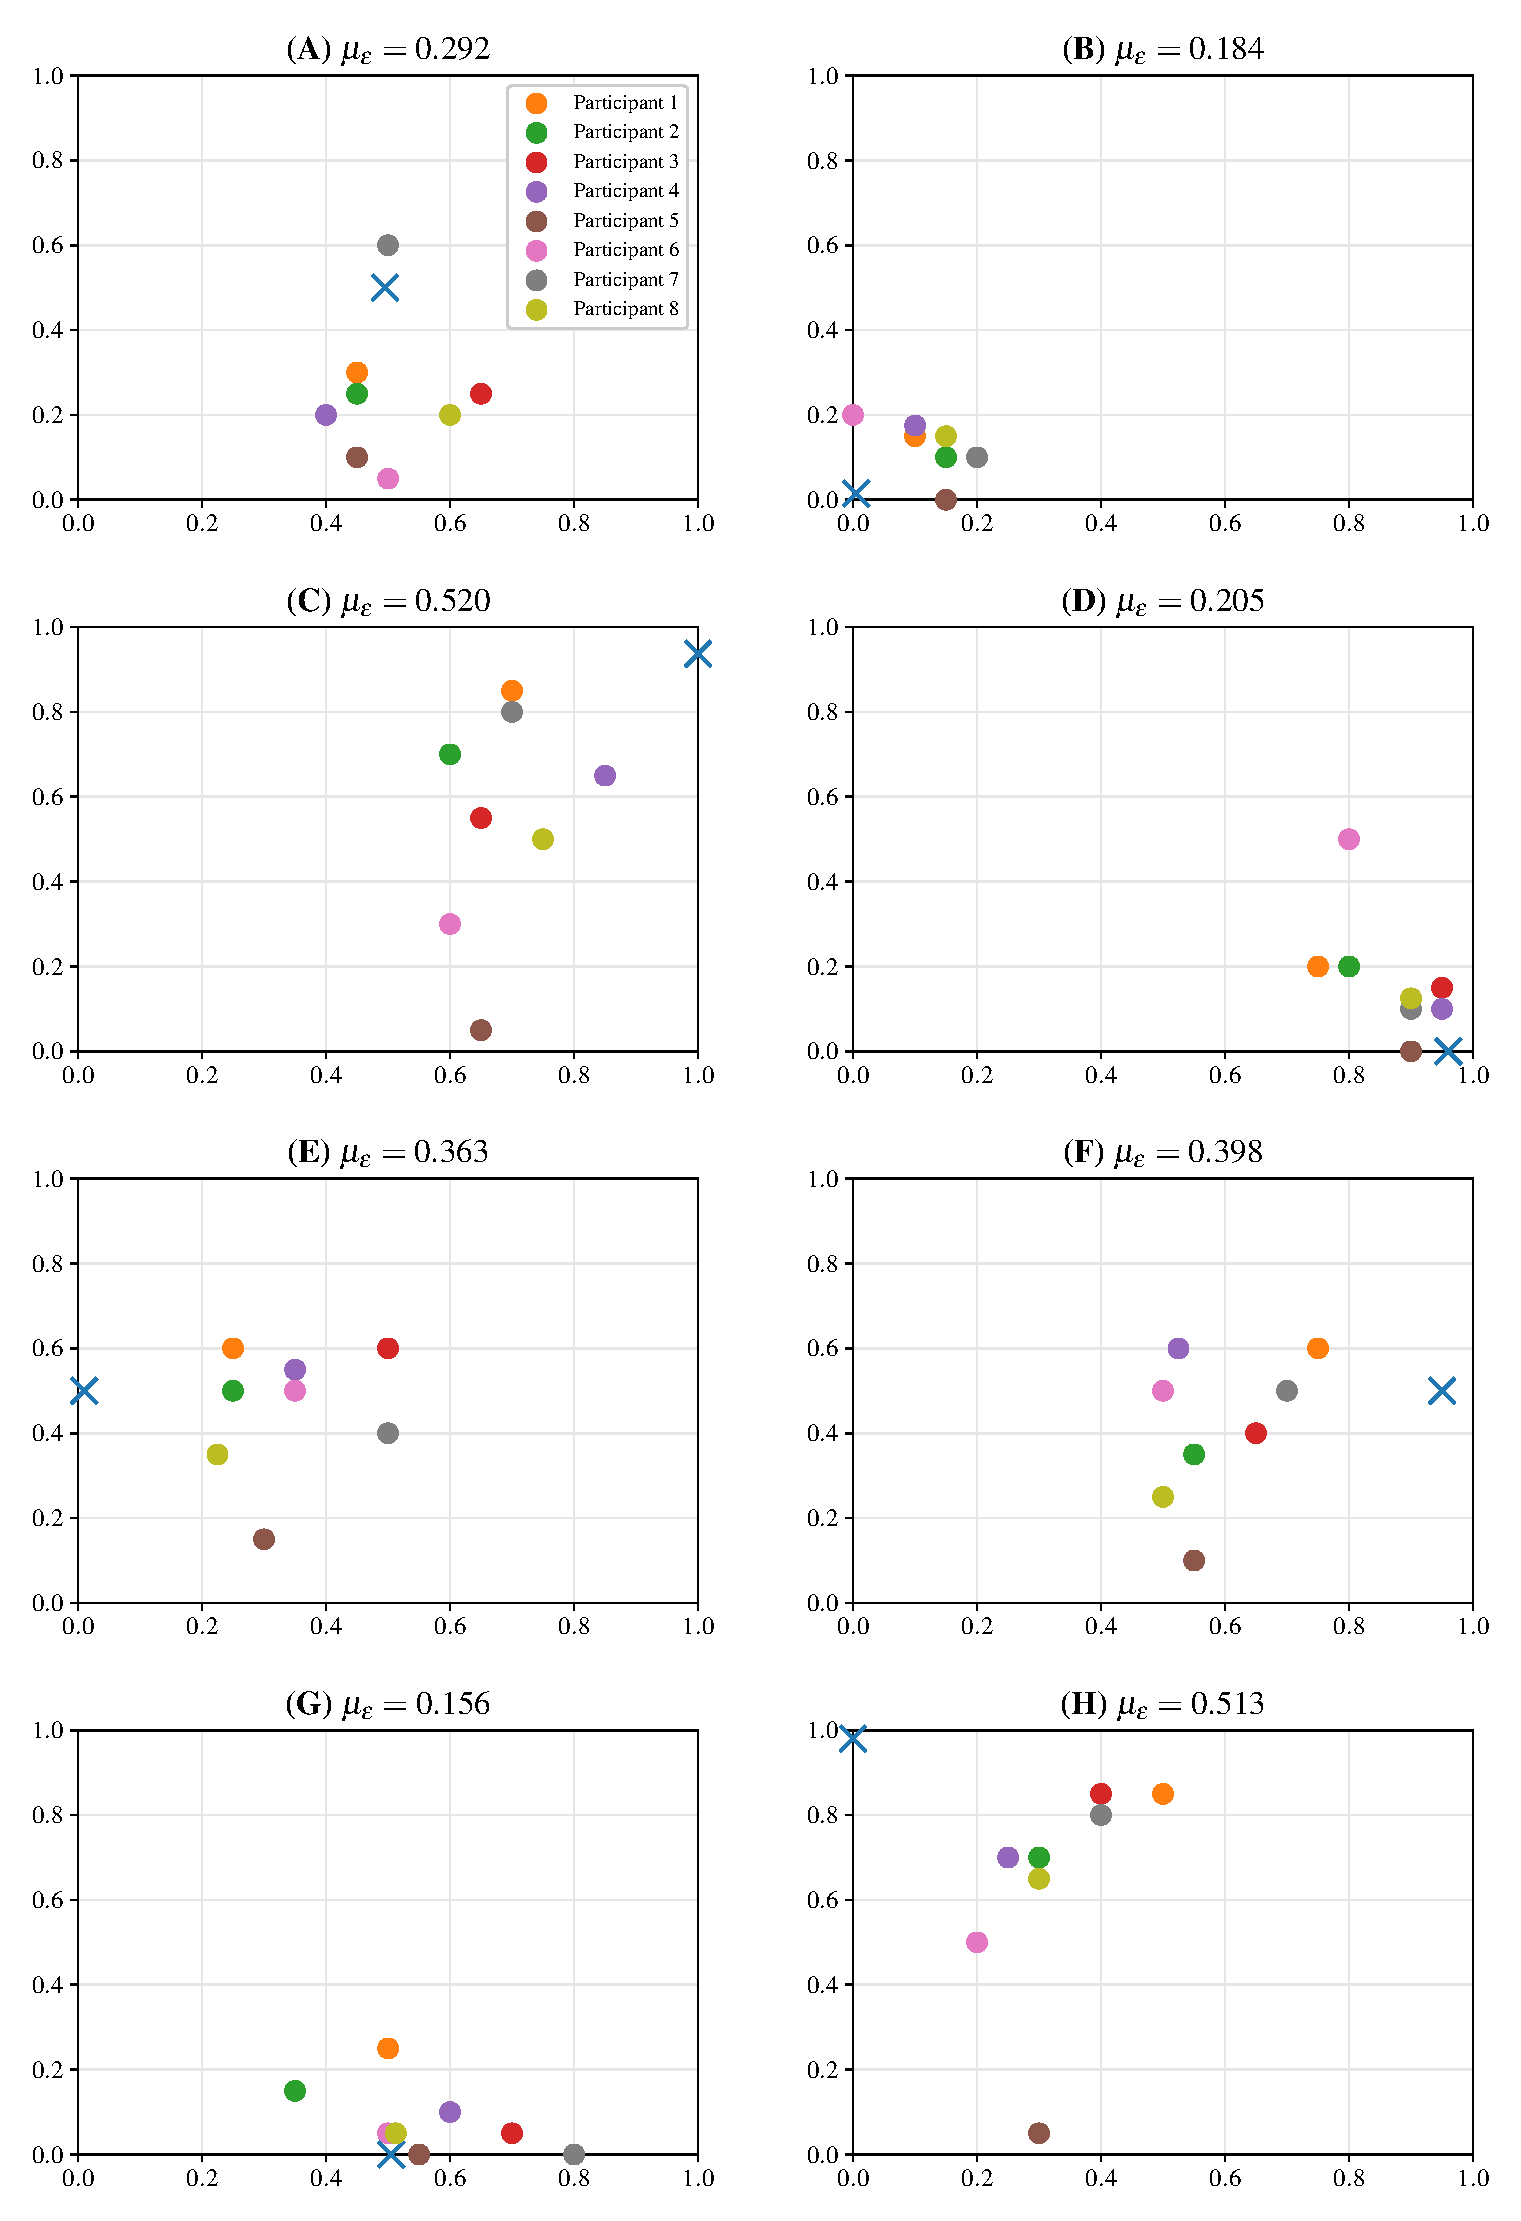
\includegraphics[width=.75\textwidth]{figures/subjective}
        \caption{
            Results of perceptual evaluation of the proposed system.
            Lateral (horizontal axis) and longitudinal (vertical axis) components
            are normalised to $[0, 1]$.
            For each plot, the horizontal axis (i.e. longitudinal component
            equalling 0) corresponds with the location of the speaker array.
            Each plot shows the intended position of the virtual sound source as
            specified by parameters to the WFS plugin interface (cross) and
            estimated sound source positions as reported by participants (dots).
            Each plot is labelled with the mean Euclidean error $\mu_\epsilon$
            between intended position and reported positions.
            Legend in plot \textbf{(A)} applies to all plots.
        }
        \label{fig:perceptual}
    \end{figure}

    The WFS system was subjected to an informal perceptual evaluation, in which
    participants were presented with a virtual sound source at various locations
    and asked to indicate, on a diagram of the virtual sound field, the point
    from which they estimated the sound had emanated.
    The informality of the experiment arose in part as a consequence of the
    listening environment not being acoustically treated, and there being sources
    of ambient sound in the laboratory in which the WFS system was installed.
    Furthermore, the speaker array (\figref{fig:eval-setup}) consisting of fifteen
    speakers, but each hardware module producing two audio output channels,
    the second channel of the right-most module was not used;
    for eight modules, however, the WFS plugin assumed a virtual sound field
    spanning sixteen speakers, thus it was possible to position a virtual sound
    source horizontally beyond the rightmost extent of the speaker array.
    Ultimately the aim of the experiment was to draw some preliminary, guiding
    conclusions as to the effectiveness of the distributed WFS system in
    triggering listeners' localisation cues, its technical and installation
    shortcomings notwithstanding.

    It was felt that listeners would be most comfortable localising a naturalistic
    sound, so, rather than use blasts of white noise as
    in~\citep[ch.~6]{verheijen_sound_1998}, and wishing to minimise the potential
    effects of frequency-dependent localisation interference due to spatial
    aliasing, a broadband stimulus was selected in the form of a close-mic recording
    of a snare drum.
    The recorded sample was repeated three times in succession at intervals of
    \qty{.125}{\s}, and, again in the interests of adding a natural quality to the
    sound, with slight variations in amplitude (the second iteration of the sample
    was played marginally quieter than the first; the third slightly louder).

    The system was presented to eight participants; a mixture of masters and PhD
    students aged between 22 and 38, with knowledge of audio and interactive
    computer systems.
    Participants were given a brief description of the system under evaluation,
    and informed that they should expect to hear sounds that appeared to emanate
    from `behind' the speaker array, from which they stood at a distance of
    $\sim$\qty{2}{\m}.
    Eight different virtual source positions were specified via automation of the
    $x$ (lateral) and $y$ (longitudinal distance) components of the position of a
    node in the WFS plugin interface.
    The range of the $x$ component corresponded with the distance from the centre of
    the driver of the leftmost speaker to that of the missing sixteenth loudspeaker;
    drivers lay at intervals of \qty{.175}{\m}, giving a horizontal axis spanning
    \qty{2.625}{\m}.
    Longitudinal position was mapped to a range from \qty{0}{\m} (i.e. lying
    directly on the speaker array) to \qty{10}{\m} `behind' the array.

    For each position, the auditory stimulus was played, and repeated at the
    participant's request.
    Each participation was five to ten minutes in duration.
    Details of the source positions for each test, and responses for the eight
    participants, are displayed in \figref{fig:perceptual}.

    As can be seen, although far from perfect, and with some significant
    outliers (e.g.\ the position reported by the fifth participant for test
    \textbf{(D)}), certain trends do appear to emerge from the results.
    Firstly, responses loosely track the intended positions, with reported
    positions most closely corresponding with intended ones for virtual source
    locations lying close to the speaker array.
    Indeed, tests \textbf{(B)}, \textbf{(D)}, and \textbf{(G)} exhibit the lowest
    mean error values between the intended and reported positions.
    The results for tests \textbf{(C)} and \textbf{(H)}, exhibit the greatest mean
    error, and ambiguity regarding the lateral position of distant sound sources is
    perhaps to be expected;
    as the distance of a sound source from the listener increases, $r_k - y_k$
    tends towards zero, and thus the ITD (and ILD) also approaches zero;
    thus, with increased distance the wavefront produced by a sound source (be it a
    real sound source or one synthesised under ideal conditions) approximates more
    and more closely a plane wave.
    In any case, despite this inherent, physical ambiguity, there is a tendency
    in results \textbf{(C)} and \textbf{(H)} toward the lateral location of the most
    longitudinally distant intended virtual source positions.
    Particularly for test \textbf{(C)}, participants seem to have had greater
    difficulty in estimating the depth of the virtual sound field; this may simply
    be as a function of their developing a familiarity with that aspect of it over
    the course of what was only a brief experiment.

    Participants were asked for any anecdotal observations they had, based on their
    experience of the experiment.
    One participant noted, for the first position in particular, that the amplitude
    variations between the snare drum strikes gave the impression of a sound source
    that was advancing upon the listening position; for the lack of any visual cue
    as to the position of the sound source, this is a reasonable conclusion to draw;
    it did not, however, ultimately prevent them from reaching a decision with
    regard to their estimate for the position of the sound source.
    Another, likely hearing the time-varying comb-filter effect, asked whether the
    ``phasing'' they were hearing was intentional.
    A third, also perceiving a similar phenomenon, suggested that they
    felt that the sound sources were moving.
    Finally, a participant with prior experience working with WFS systems, remarked
    that the distance effect (i.e.\ the WFS prefilter) was perhaps a little extreme,
    and not altogether realistic.

    \subsubsection{Discussion}\label{subsubsec:discussion-percep}

    The phasing effect noted by one participant is a consequence of the approach
    taken to combating jitter and keeping the clients close, temporally, together,
    and as close to the server as possible.
    It is clear that the current approach is, at best, too aggressive to be viable
    for high-quality audio output.
    Furthermore, an unpitched sound source like a snare drum, though audibly
    susceptible to the time-varying comb-filter effect described, masks other
    artefacts caused by phenomena such as rapid fluctuations in the clients' buffer
    read position increment, and sudden, comparatively large audio clock
    adjustments.

    The above being said, the perceptual test indicates that the system produces
    virtual sound sources that listeners are, at least to some extent, able to
    localise.
    Further, it achieves this at a significantly lower cost-per-channel than any of
    the systems discussed in sections \secref{subsubsec:spatial-sota}, and, speakers
    and cables excepted, compares favourably with the OTTOSonics system referred to
    in \secref{subsec:distributed-audio-systems}, particularly as channel-count
    increases, i.e.\ in terms of cost, it has the potential to scale better.
    The most costly component of the system is the computer, but this could be
    exchanged for any interested user's personal machine, so long as it is able to
    run a DAW and has an ethernet interface.
    The Teensy modules, including audio shield, cost around \texteuro{45};
    eight-port ethernet switches can be purchased for as little as \texteuro{20-30}.
    Assuming a computer costing \texteuro{1500}, at 16 channels we can estimate
    around \texteuro{120}/channel, dropping to \texteuro{50}/channel for 64
    channels.


    \section{Conclusion}\label{sec:conclusion}

    In this article we have described an exploration of transmission of audio data
    over computer networks, distributed computing and audio spatialisation.
    A networked audio system was developed, strategies devised for
    addressing challenges presented by distributed computing, and a distributed
    spatial audio system was developed and deployed.
    Evaluation of the system exposed the extent of the technical challenges
    that confront it in its current form, and shed light on opportunities for
    further development.
    Perceptual testing revealed that it may offer performance sufficient to support
    timing-critical sound field synthesis techniques.
    The proposed system represents a milestone on the road towards an accessible
    alternative to state of the art spatial and immersive audio installations.

    It has been shown that a system of discrete computational entities can
    communicate effectively over an ethernet network, exchanging audio and control
    data in a scalable fashion via a UDP multicast group.
    Though facing significant technical challenges, the foundational requirements of
    such a system have been demonstrated, with encouraging results with regard to
    spatial audio applications.

    Timing discrepancies between entities in the networked audio system give rise
    to audible artefacts such as time-varying comb-filtering.
    Loss of synchronicity is difficult to measure and compensate for in real-time;
    the extent of the resulting audible disturbances is unpredictable, and firmer
    conclusions about their extent, and thresholds for their perceptibility should
    ideally be sought.
    The developed strategies for mitigation of asynchronicity call for further
    refinement, but even in their current form support the creation of localisable
    WFS virtual sound sources.

    Given its potential to disrupt the present situation with regard to spatial
    audio installations, or complement it with a modular approach that could serve
    more flexible and creative ends, it is hoped that scope will exist to develop
    this work further.
    A number of technical challenges remain, and questions with regard to the
    fundamental characteristics of the various components of the devised system
    stand unanswered.
    From the level of audio hardware and driver software, to audio host and audio
    buffer behaviour, to network QoS and the performance of network switches, to
    the behaviour of the hardware platform, its processor and audio codec, plus its
    software libraries \textemdash{} much that is typically taken for granted in the
    development of embedded systems, and audio and networking applications, calls
    for deeper investigation.

    Each microcontroller generates a clock signal to deliver to its audio shield,
    which, in a locally distributed setting, is rather redundant.
    It may be possible to generate a single, authoritative clock on one node and
    deliver that to all others in the system.
    If this can be achieved, it would remedy the issue of clock drift, leaving only
    jitter to be addressed.
    Furthermore, Teensy is not the only platform worthy of consideration;
    developments in microcontroller technology are to be expected, and suitable
    devices supporting higher-quality audio than offered by Teensy may emerge.
    One device considered only briefly here is the Raspberry Pi;
    in principle it is priced comparably with the Teensy, and is supported by audio
    breakout boards that can output 24-bit audio.
    Improved bare metal support, including the creation of a \texttt{faust2circle}
    tool, could make Raspberry Pi a significantly more attractive platform,
    particularly in terms of memory and the dimensions of the sound fields that
    could be synthesised.

    With regard to audio spatialisation, a basic, linear, wave field synthesis
    algorithm has been demonstrated here, implementing virtual primary sources.
    WFS is capable of producing other types of sources, supporting nonlinear
    speaker arrays, three-dimensional arrays, and more faithful models of
    energy loss due to absorption.
    There are many further avenues to pursue, including optimising any DSP
    algorithms to best exploit the capabilities of what, in the shape of the
    Teensy and other microcontroller systems, are very powerful platforms.
    Further, and only given cursory treatment here, higher order ambisonics, subject
    to an assessment of its suitability to parallelisation, remains as a worthy
    target for implementation in future work.

    % As per https://www.frontiersin.org/Design/pdf/Frontiers_Journal_style_table.pdf
    \bibliographystyle{Frontiers-Harvard}
    \bibliography{NetworkedAudio}
    %%% Make sure to upload the bib file along with the tex file and PDF

\end{document}
